%
% LaTeX report from the 2020 PHIMECA internship 
%
\documentclass[a4paper,10pt]{article}
\usepackage{graphicx}
\usepackage[english]{babel}
\usepackage[utf8]{inputenc}
\usepackage[T1]{fontenc}
%\usepackage{apacite}
\usepackage{float}
\usepackage[section]{placeins}
\usepackage{mwe}
\bibliographystyle{apalike}
\usepackage{hyperref}
\usepackage{amsmath}
\usepackage{mathtools}
\usepackage{gensymb}
\usepackage[toc,page]{appendix}

\begin{document}
%
   \title{Rapport de stage PHIMECA}

   \author{Kristof Attila Simady \\ e-mail: kristof.simady@sigma-clermont.fr}
          
   \date{05/03/2020}

   \maketitle
   
   \tableofcontents
 
  \newpage
    
\section*{Avant propos}

Le cadre d'étude offert par SIGMA Clermont a donné la possibilité d’effectuer une année supplémentaire de stages pour étoffer nos connaissances scientifiques et techniques  et découvrir le monde industriel comme des culture étrangères.
De par mon appétence pour la recherche et l'informatique, j'ai eu la chance de pouvoir venir effectuer mon stage au sein de l'entreprise \textbf{PHIMECA}, située à Clermont-Ferrand, et depuis longtemps en partenariat avec SIGMA. \\

Il aura été l'occasion pour moi de développer un ensemble de savoir pointus sur l'analyse fiabiliste et les différents outils employés, tout comme d'avoir pu travailler sur un projet de recherche industriel complexe et s'étalant sur une multitude de domaines scientifiques. En plus d'avoir pu me servir des connaissances acquises au cours de ma formation, et approfondir ces dernières, l'utilisation de l'outil informatique et son harmonisation avec les méthodes d'analyse a permis d'acquérir de la fluidité de travail et d'ouvrir l'accès à un grand nombre d'outils, puisque plus on travaille avec des outils informatiques différents, plus l'acquisition d'une nouvelle compétence informatique devient rapide et peu coûteuse en énergie. \\

Bien sur, tout cela n'aurait pas été possible sans le cadre offert par Phimeca et la liberté d'action dont on jouit en travaillant ici. En effet, bien qu'ayant un sujet assez défini, la responsabilité quant à l'avancement sur le projet, ou encore le choix des outils a utiliser et la méthodologie a employer était des choix à faire soi même. Ce type de liberté d'action implique d'avoir suffisamment de connaissances pour envisager les différentes méthodes de résolution possibles et parvenir à choisir la bonne, et cela implique encore plus d'arriver a rapidement se familiariser seul avec un outil ou domaine de recherche et acquérir suffisamment d'informations sur celui-ci pour parvenir soit à l'employer, soit a juger de sa pertinence dans le projet. \\

En plus de ce cadre de travail et ce projet formateur, l'ambiance agréable au sein de \textbf{PHIMECA} et la présence d'une équipe assez jeune ont rendu ce stage très agréable et motivant. \\

Je souhaite donc avant tout remercier Mr. Nicolas GAYTON, qui a rendu ce stage possible grâce a ses nombreuses années d'échange et de collaboration avec \textbf{PHIMECA}, et la confiance qu'il a porté en mes capacités à évoluer dans ce milieu de travail et m'avoir proposé en tant que stagiaire.\\

Je souhaite ensuite remercier Mr. Antoine DUMAS, mon tuteur et responsable de l'équipe FIC (Fiabilité Incertitudes Cournon), qui a su trouver un sujet de stage intéressant et formateur, me mettre sur les bonnes pistes
des que des difficultés apparaissaient et qui a su enfin m'accorder suffisamment de confiance pour aller représenter l'implication de \textbf{PHIMECA} dans ce projet face aux autres acteurs impliqués. \\

Mes remerciements vont ensuite à Mr. Thierry YALAMAS, qui a su m'introduire à l'équipe et la philosophie d'entreprise, et qui a veillé à ce que l'ambiance de travail soit toujours la plus propice aux idées innovatrices et à l'épanouissement de chacun, même dans le cas de force majeure qu'a été cette épidémie de COVID-19. \\

Je remercie enfin le reste de l'équipe, Oussama B., Fabien T., Julien S. Marc G., Rémi P., Guillaume G., Céline D. , Nathalie G., et tout les autres ... (à suivre)

\paragraph{Note:}
Ce document est autant un rapport de stage qu'une note à qui voudrait se servir des différentes méthodes explorées et codes développés.

\newpage
\section{Premiers 5 mois de stage}
\subsection{Introduction}
Dans le cadre d'analyse probabiliste et fiabiliste, il est d'usage d’effectuer des analyses de sensibilité sur une ou plusieurs grandeurs d’intérêt, grâce à divers moyens comme les indices de Sobol' ou les analyses de corrélation. \\
Ces analyses sont néanmoins souvent cantonnées à des modèles n'ayant en sortie et entrée que des grandeurs scalaires, pour lesquelles de nombreuses méthodes existent dans la littérature.\\
L'objectif du travail présenté ici, est d’effectuer ce type d'analyse sur des modèles ayant en entrée plusieurs champs aléatoires et des variables aléatoires scalaires et en sortie aussi des champs et grandeurs scalaires. \\ Pour compléter cela, il était bien sûr aussi demandé de d'abord créer un modèle simple gouverné par des champs stochastiques et de faire de l'analyse de sensibilité sur ce modèle. \\
Il sera d'abord présenté différentes méthodes présentes dans la littérature, avec leurs potentiels avantages et défauts. \\ 
Cette approche des l'analyse de sensibilité nous renvoie aussi sur des champs de recherche bien différents, car les méthodes peuvent autant venir du champ de la mécanique que de la géologie ou l'étude environnementale.

 
\subsection{Recherche bibliographique}
Ce travail de recherche a été l'occasion de parcourir un grand nombre de travaux, liés de plus ou moins loin à l'analyse de sensibilité sur des processus gaussiens.\\
On notera notamment les travaux de \cite{Lilburne2009Feb} qui donnent dans leur travail un état de l'art complet sur les différentes méthodes utilisables pour l'analyse de sensibilité sur champs gaussiens. \\
D'autres techniques plus récentes ont néanmoins vu le jour, et ce sont ces dernières que nous avons explorés en premier. Notamment les travaux de \cite{Wei2017May} sur l'analyse de sensibilité de structures ayant en entrée des variables aléatoires et processus stochastiques variant dans le temps, ou encore le travail de \cite{Pronzato2019Jul} qui développe un métamodel entre l'entrée et sortie d'un modèle gouverné par des champs stochastiques.

\subsubsection{Travaux retenus}
Etant donné que les missions d'analyse de sensibilité et d'incertitudes se font classiquement en se basant sur la bibliothèque \textit{openTURNS} développé par PHIMECA, le choix a été fait d'adapter techniques de recherche et méthodes déja existantes dans l'API au problème étudié. 


\subsubsection{Methodes et outils de travail}
L'ensemble des codes ont été écrits dans le langage \textit{Python}, en se servant majoritairement des bibliothèques a caractère scientifique (\textit{SciPy, NumPy}) et la bibliothèque développée en partie par \textbf{PHIMECA :} \textit{openTURNS} (\emph{open treatment of Uncertainties and Risk \& Statistics })\cite{OpenTURNS}.\\
\textbf{PHIMECA} a fourni un poste de travail Linux, tout comme un accès au serveur de calcul pour les modèles un peu plus conséquents. \\

\subsection{Analyse de la problématique, premier tests et prise en main des outils}

\subsubsection{Mission confiée et tâches associées}
L'objectif du stage était de développer une méthodologie pour l'analyse de sensibilité sur des modèles gouvernés par des champs aléatoires (Champs Stochastiques) et des variables aléatoires, et qui en sortie sont aussi représentables par une collection de champs et variables aléatoires. \\
Plus spécifiquement, cette méthodologie était à appliquer à un modèle d'échangeur de chaleur air-air commercialisé par \textbf{LIEBHERR} et utilisé pour la régulation thermique de l'air ambiant dans les avions de ligne.\\\\
Comme la mission confiée au sein de \textbf{PHIMECA} se rapprochait d'un travail de recherche, celui -ci était bien sur accompagné de nombreuses étapes distinctes. En effet, en plus du développement des codes et de l'application analytique, une recherche bibliographique a du être menée en amont pour parvenir a lister les différentes méthodes d'analyse existantes et tester celles qui pourraient convenir au mieux. De plus, une phase d'apprentissage et de tests a du d'abord être nécessaire pour parvenir à prendre en main les différents outils, et comprendre la théorie et les mathématiques sous-jacentes.\\

\subsubsection{Prise en main d'openTURNS et de la théorie sur les champs stochastiques}
\paragraph{Champs Stochastiques\\} 
Un champ stochastique est un champ de variables aléatoires toutes corrélées entre elles, et dont l'intensité de la corrélation est déterminée par leur proximité dans l'espace. Par exemple la position de tout objet est corrélée à sa position aux intervalles de temps proches (continuité du temps), ou bien les températures au dessus d'un pays sont corrélés à faible distance mais l'effet aléatoire est plus présent lorsque les distances sont importantes. \\
Ce type de modélisation des champs est couramment utilisée pour modéliser des propriétés présentant des variabilités gaussiennes mais une continuité dans leur espace de définition. \\ Lorsque la corrélation est seulement dépendante de la distance entre deux points de l'espace et non d'une position absolue, on parle d'un champ stationnaire. Lors de cette étude, on se place dans ce cas.\\ 

\newpage

\begin{figure}[H]
   \centering   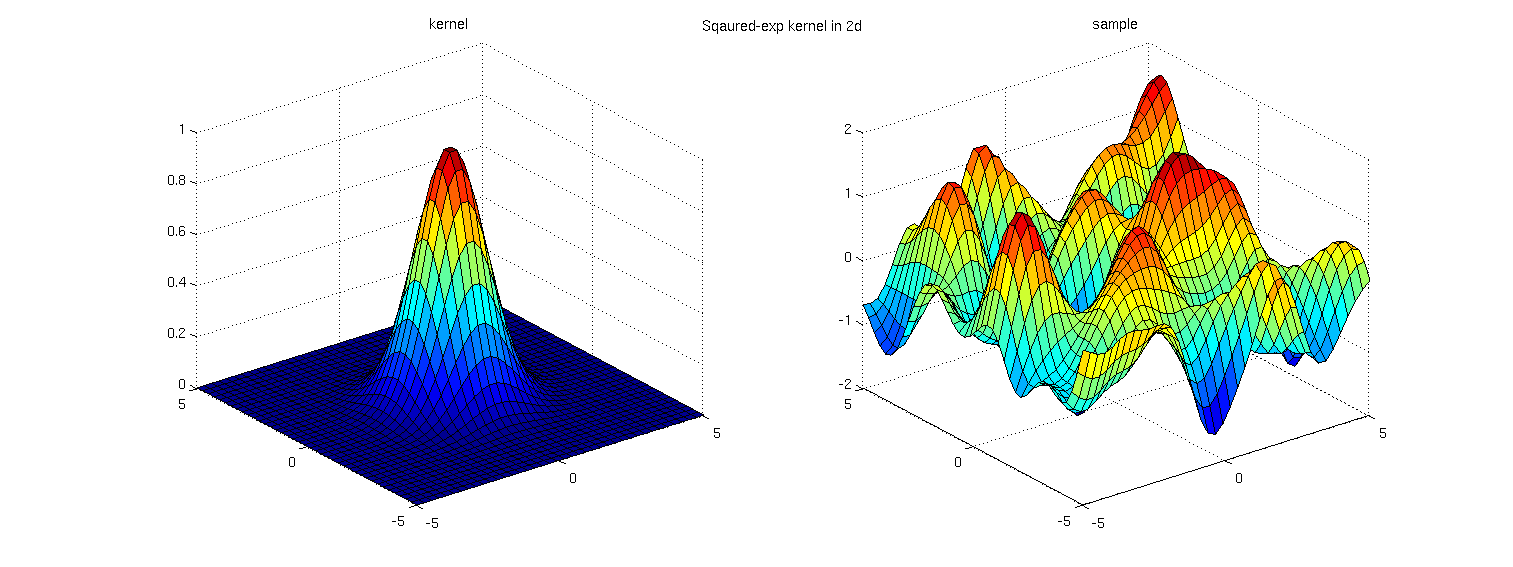
\includegraphics[scale=0.25]{stochastic_process2d.png}
      \caption{Réalisation d'un champ stochastique en deux dimension. Le champ est continu dans l'espace et la primitive est une gaussienne en deux dimensions.}
         \label{realChamp}
\end{figure}

Mathématiquement, cette corrélation peut être définie par différents modèles. Les deux modèles de corrélation les plus simples sont les fonctions de covariance exponentielles (1) et les exponentielles quadratiques (2).  

   \begin{eqnarray}
      				C(d) & = & \exp(-d/V)\\
                    C(d) & = & \exp(-(d/V)^{2});
   \end{eqnarray}
   
Avec \emph{V} étant le paramètre d'échelle et \emph{d} la norme euclidienne de la distance entre deux points de l'espace considéré.\textit{(plus le paramètre d'échelle est grand, plus le champ est lissé, tout comme le modèle quadratique est aussi plus lisse)}\\
Une autre fonction de covariance, celle de \emph{Matérn}, est aussi très utilisée, puisqu'elle présente des comportements limites similaires aux deux fonctions exponentielles présentes plus haut. La dérivabilité de ce modèle est réglable via le paramètre $\nu$, ainsi la régularité du champ est facilement modifiable.

   \begin{eqnarray}
C_{v}(d) & = & \sigma^{2}\frac{2^{1-\nu}}{\Gamma(\nu)}\left(\sqrt{2\nu}\frac{d}{\rho}\right)^{\nu}K_{\nu}\left(\sqrt{2\nu}\frac{d}{\rho}\right);
   \end{eqnarray}\\

La continuité des processus gaussiens et leur comportement quasi ondulaire, permet de les traiter de manière un peu analogue à la décomposition de fourrier, et des les décomposer en une somme infinie de variables aléatoires gaussiennes décorrélées.. Cette méthode de décomposition vient du théorème de \emph{Karhunen-Loève}. \\
La construction de cette série infinie se fait grâce aux vecteurs propres issus de la matrice de corrélation du modèle, et grâce à une base de vecteurs orthonormaux dans un espace Hilbertien. Les détails mathématiques de cette méthode peuvent être trouvées en  \cite{Sudret2000Jan}. \\
Lors de l’approximation de \emph{Karhunen-Loève}, la série est tronquée à l'ordre \textbf{M}.
%Approximation de Kahrunen Loeve 
   \[
      \begin{array}{lp{0.8\linewidth}}
         H(\textbf{x}, \theta) & Approx. Procéssus Gaussien \\
         \lambda_{i}          & Valeur Propre de la matrice de covariance \\
         \xi_{i}             & Variable Normale Centrée Réduite \\
         \varphi_{i}(\textbf{x}) & Vecteur propre de la matrice de covariance
      \end{array}
   \]
   \begin{eqnarray}
H(\textbf{x}, \theta) & = & \sum_{i=1}^{M}\sqrt{\lambda_{i}}\xi_{i}(\theta)\varphi_{i}(\textbf{x});
   \end{eqnarray}\\

Cette décomposition permet de représenter l'ensemble de variabilité du champ avec des variables gaussiennes décorrélées, et donc de faire des analyses de sensibilités sur cette nouvelle représentation du champ.

\paragraph{openTURNS\\}
\emph{openTURNS} est initialement un projet de bibliothèque open-source pour le traitement des incertitudes et des risques, commun a trois entreprises fondatrices, \textbf{Airbus}, \textbf{EDF} et \textbf{Phimeca Engineering}, projet ayant débuté en 2005. \\
Depuis, deux autres organismes, \textbf{IMACS} et l'\textbf{ONERA} ont rejoint le développement d'\emph{openTURNS}, qui se révèle être un grand atout pour le traitement des incertitudes et l’ingénierie fiabiliste.
En effet, le projet d'\emph{openTURNS} est un regroupement d'un ensemble d'algorithmes performants écrits en C++, se basant sur la théorie développée pour les traitement des incertitudes, l'optimisation robuste, et les études de sensibilité.\\ 
Un \textit{wrapper}\footnote{Un wrapper ou fonction wrapper, est un programme qui appelle un autre programme. Il permet entre autres d'utiliser du code dans un milieu hétérogène, ici, du C++ depuis Python} a été utilisée pour lier l'ensemble de la bibliothèque C++ à un module Python, et de pouvoir profiter de la facilité d'utilisation du langage Python et de sa flexibilité, tout en gardant les vitesses d’exécution du C++.\\
\textbf{PHIMECA} développe des logiciels commerciaux en se basant sur le module \emph{openTURNS}, qui sont plus ergonomiques dans leur utilisation et automatisent certaines parties moins évidentes en utilisation directe de la librairie. \\
Néanmoins, la librairie reste quand même extrêmement bien documentée, avec la théorie mathématique sous-jacente à chaque algorithme d'explicitée, tout comme de nombreux exemples. La documentation présente de même des cas d'applications précis montrant la logique à avoir lors de l'écriture de codes avec \emph{openTURNS}.
\newpage


\subsection{Exemple théorique simple, premiers codes}
Pour parvenir a tester les méthodes trouvées lors de la recherche bibliographique, et avoir un modèle simple et rapide à exécuter, un exemple simple a été développé : 
Il s'agit d'un modèle de poutre en appui sur ses deux extrémités
\begin{figure}[H]
   \centering   
   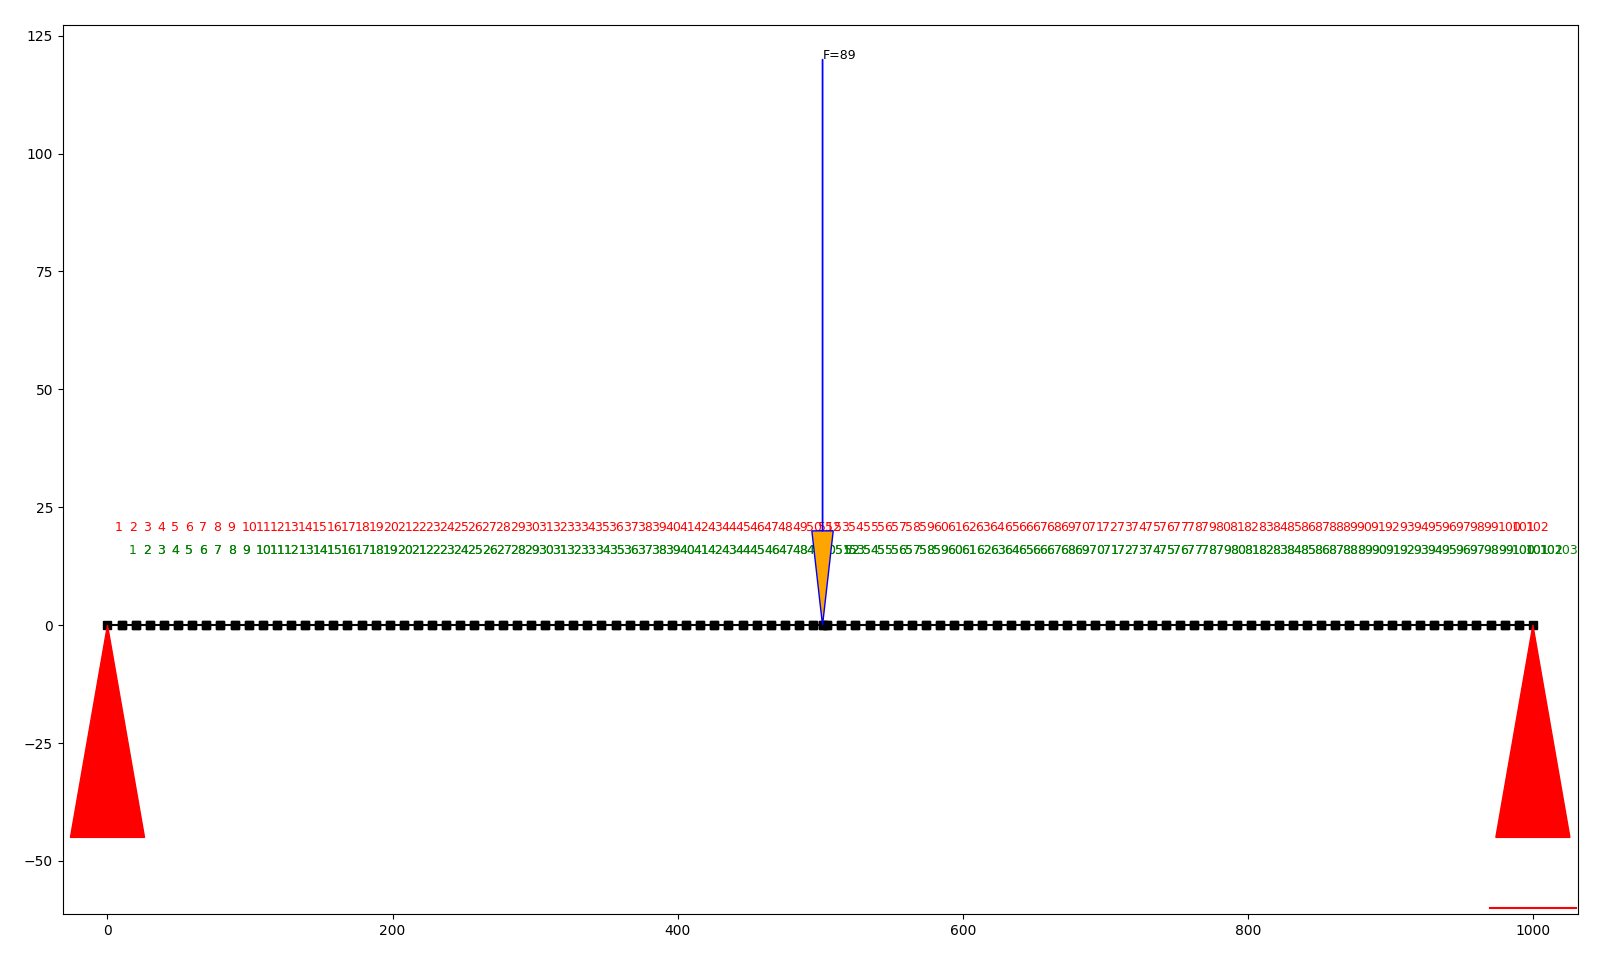
\includegraphics[scale=0.20]{beam_structure.png}
      \caption{Modélisation d'une poutre en appui sur ses deux extrémités avec la bibliothèque anastruct}
         \label{fig:nonfloat}
\end{figure}

La particularité de ce modèle de poutre est, en plus d'être une aberration physique, le fait que le diamètre et le module de young sont gouvernés par un processus gaussien en une dimension, suivant la longueur de la barre. Pour parvenir à modéliser cette variation, le modèle est bien-sûr subdivisé en une centaine d'éléments finis, et le champ discrétisé sur un maillage de même longueur.\\
En plus de ces deux grandeurs gouvernées par des champs, la densité du matériau, la position de la force, et la norme de la force sont représentés par des variables aléatoires Gaussiennes. Cette modélisations'est faite avec l'excellente bibliothèque \textbf{\textit{Anastruct}} de \cite{Vink2020Feb}.

\begin{figure}[H]
   \centering   
   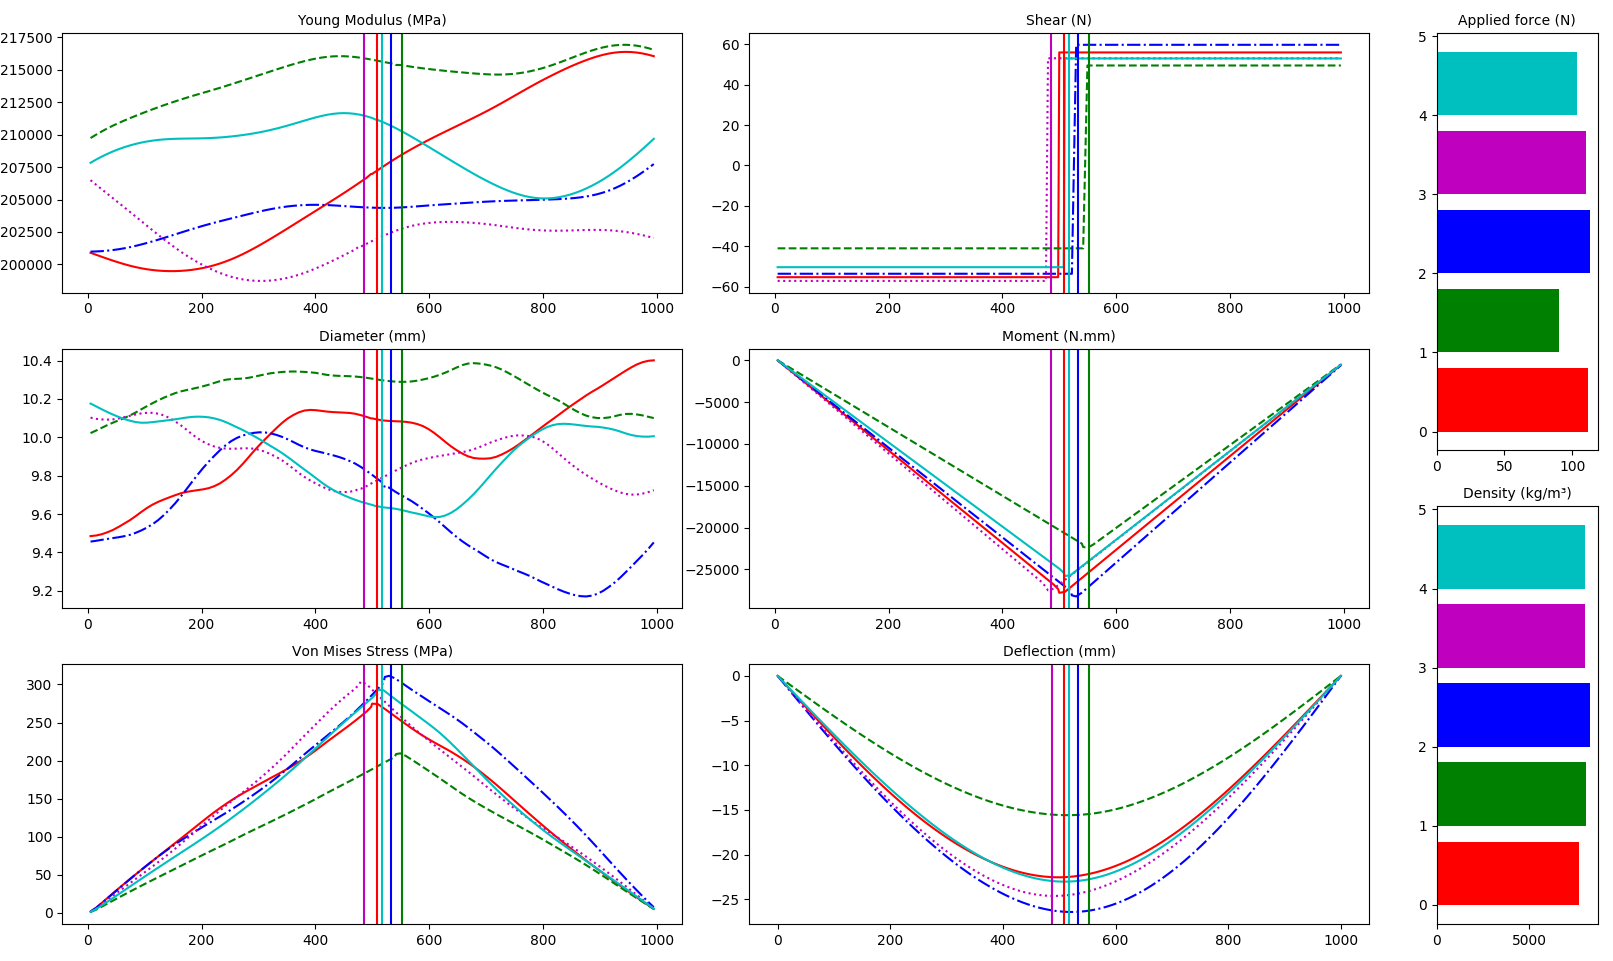
\includegraphics[scale=0.33]{beam_experience.png}
      \caption{Échantillon de 5 réalisations de la poutre en flexion. [Sur la gauche : Processus gouvernant le module de young, Processus gouvernant le diamètre, contrainte de Von Mises] | [Sur la droite : Contrainte de cisaillement, moment de flexion, déflexion] }
         \label{beamExperience}
\end{figure}

Les grandeurs d'étude choisies ici sont la contrainte de Von Mises, la déflection de chaque noeud, et la déflection maximale. On pourrait de même choisir une contrainte de Von Mises maximale pour représenter la défaillance. 

Comme chacun des processus stochastiques peut être décomposé en une somme finie de variables aléatoires normales grâce à la décomposition de karhunen-Loeve, l'on peut à l'inverse, générer des champs stochastiques à partir d'une collection de variables aléatoires, dont les paramètres sont issus de l'analyse même du champ.

On considère donc notre modèle plus comme fonction de variables aléatoires et de processus stochastiques, mais seulement comme une fonction de variables aléatoires scalaires.

Ceci permet de faire l'analyse de sobol classique (avec l'algorithme de sensibilité de \textit{Saltelli}) sur ces nouvelles variables aléatoires.

La difficultée ici, est d'ensuite relier les indices de sensiblité de Sobol des variables aléatoires définissant le champ au champ stochastique même. (On ne souhaite n'avoir qu'un seul indice de sobol pour un champ.) 

\subsubsection{Choix des codes et difficultées algorithmiques}
Au vu de choix de développer une méthode algorithmique pour l'analyse de sensiblité sur des champs stochastiques, et non pas de juste faire l'analyse de sensibilité sur une seule problématique, il y avait un besoin de robustesse supplémentaire pour l'écriture des différents codes. Ces derniers doivent pouvoir fonctionner avec tout type de fonction en python prennant en entrée des champs et variables aléatoire, et renvoyant un tuple de variables aléatoires. 

Pour pouvoir tester ceci, l'exemple de la poutre en éléments fins à été codée à part, et peut être utilisée directement comme fonction, indépendamment de l'analyse de sensibilité. Cette dernière prend de même en entrée deux champs stochastiques et trois variables aléatoires, et peut renvoyer plusieurs arguments. Les tests ont été faits avec la fonction ne renvoyant qu'une collection de champs (contraintes de von mises) et avec la fonction renvoyant un tuple (collection de champs + vecteur déflection maximale). Ce choix augmente le nombre de vérification qu'il y a à effectuer au sein du code, mais permet l'utilisation d'un plus grand nombre de fonctions, et l'analyse de sensiblité sur l'ensemble des variables de sortie en une seule fois.

Pour parvenir à bien controller les processus stochastiques, une classe a été écrite \textit{NdGaussianProcessConstructor}, qui permet de définir entièrement un processus stochastique, et possède de nombreuses méthodes pour créer des échantillons, faire les décompositions de Karhunen-Loeve, ou encore reconstituer un champ à partir de la dite décomposition. Enfin, comme les échantillons sont nécessaires pour la décomposition de Karhunen-Loeve, et que ceux-ci peuvent être de taille plutôt importante, ils sont enregistrés sous form de \textit{numpy.memmap} dans un fichier temporaire, pour relacher un peu de pression sur la mémoire vive.\\

En interne, le modèle fonction de champs stochastiques, passe par un wrapper qui fait qu'on peut la considerer comme seulement fonction de variables aléatoires gaussiennes. Cela permet d'utiliser les méthodes internes à openturns comme l'algorithme de Saltelli pour estimer les indices de sobol. \\
\newpage
Néanmoins, pour pallier certaines difficultées comme les fonctions qui par moment renvoient des \textbf{\textit{np.nan}} (donc lorsqu'il y a eu une erreur), on passe d'abord par une étape de correction:  l'ensemble des valeurs de sortie contenant des \textit{nan} sont regénérées, et comme les entrées de l'étude sont des combinaison de deux ensembles de variables aléatoires A et B, toutes les autres permuttations des entrées ayant entrainé des erreurs sont supprimées et remplacées. Cette étape est éxpliquée en figure \ref{posprocessing} \

Les codes sont accessibles via \textit{\textbf{github}}: \\
\url{https://github.com/Kramer84/stochastic_process_analysis}

\begin{figure}[H]
   \centering   
   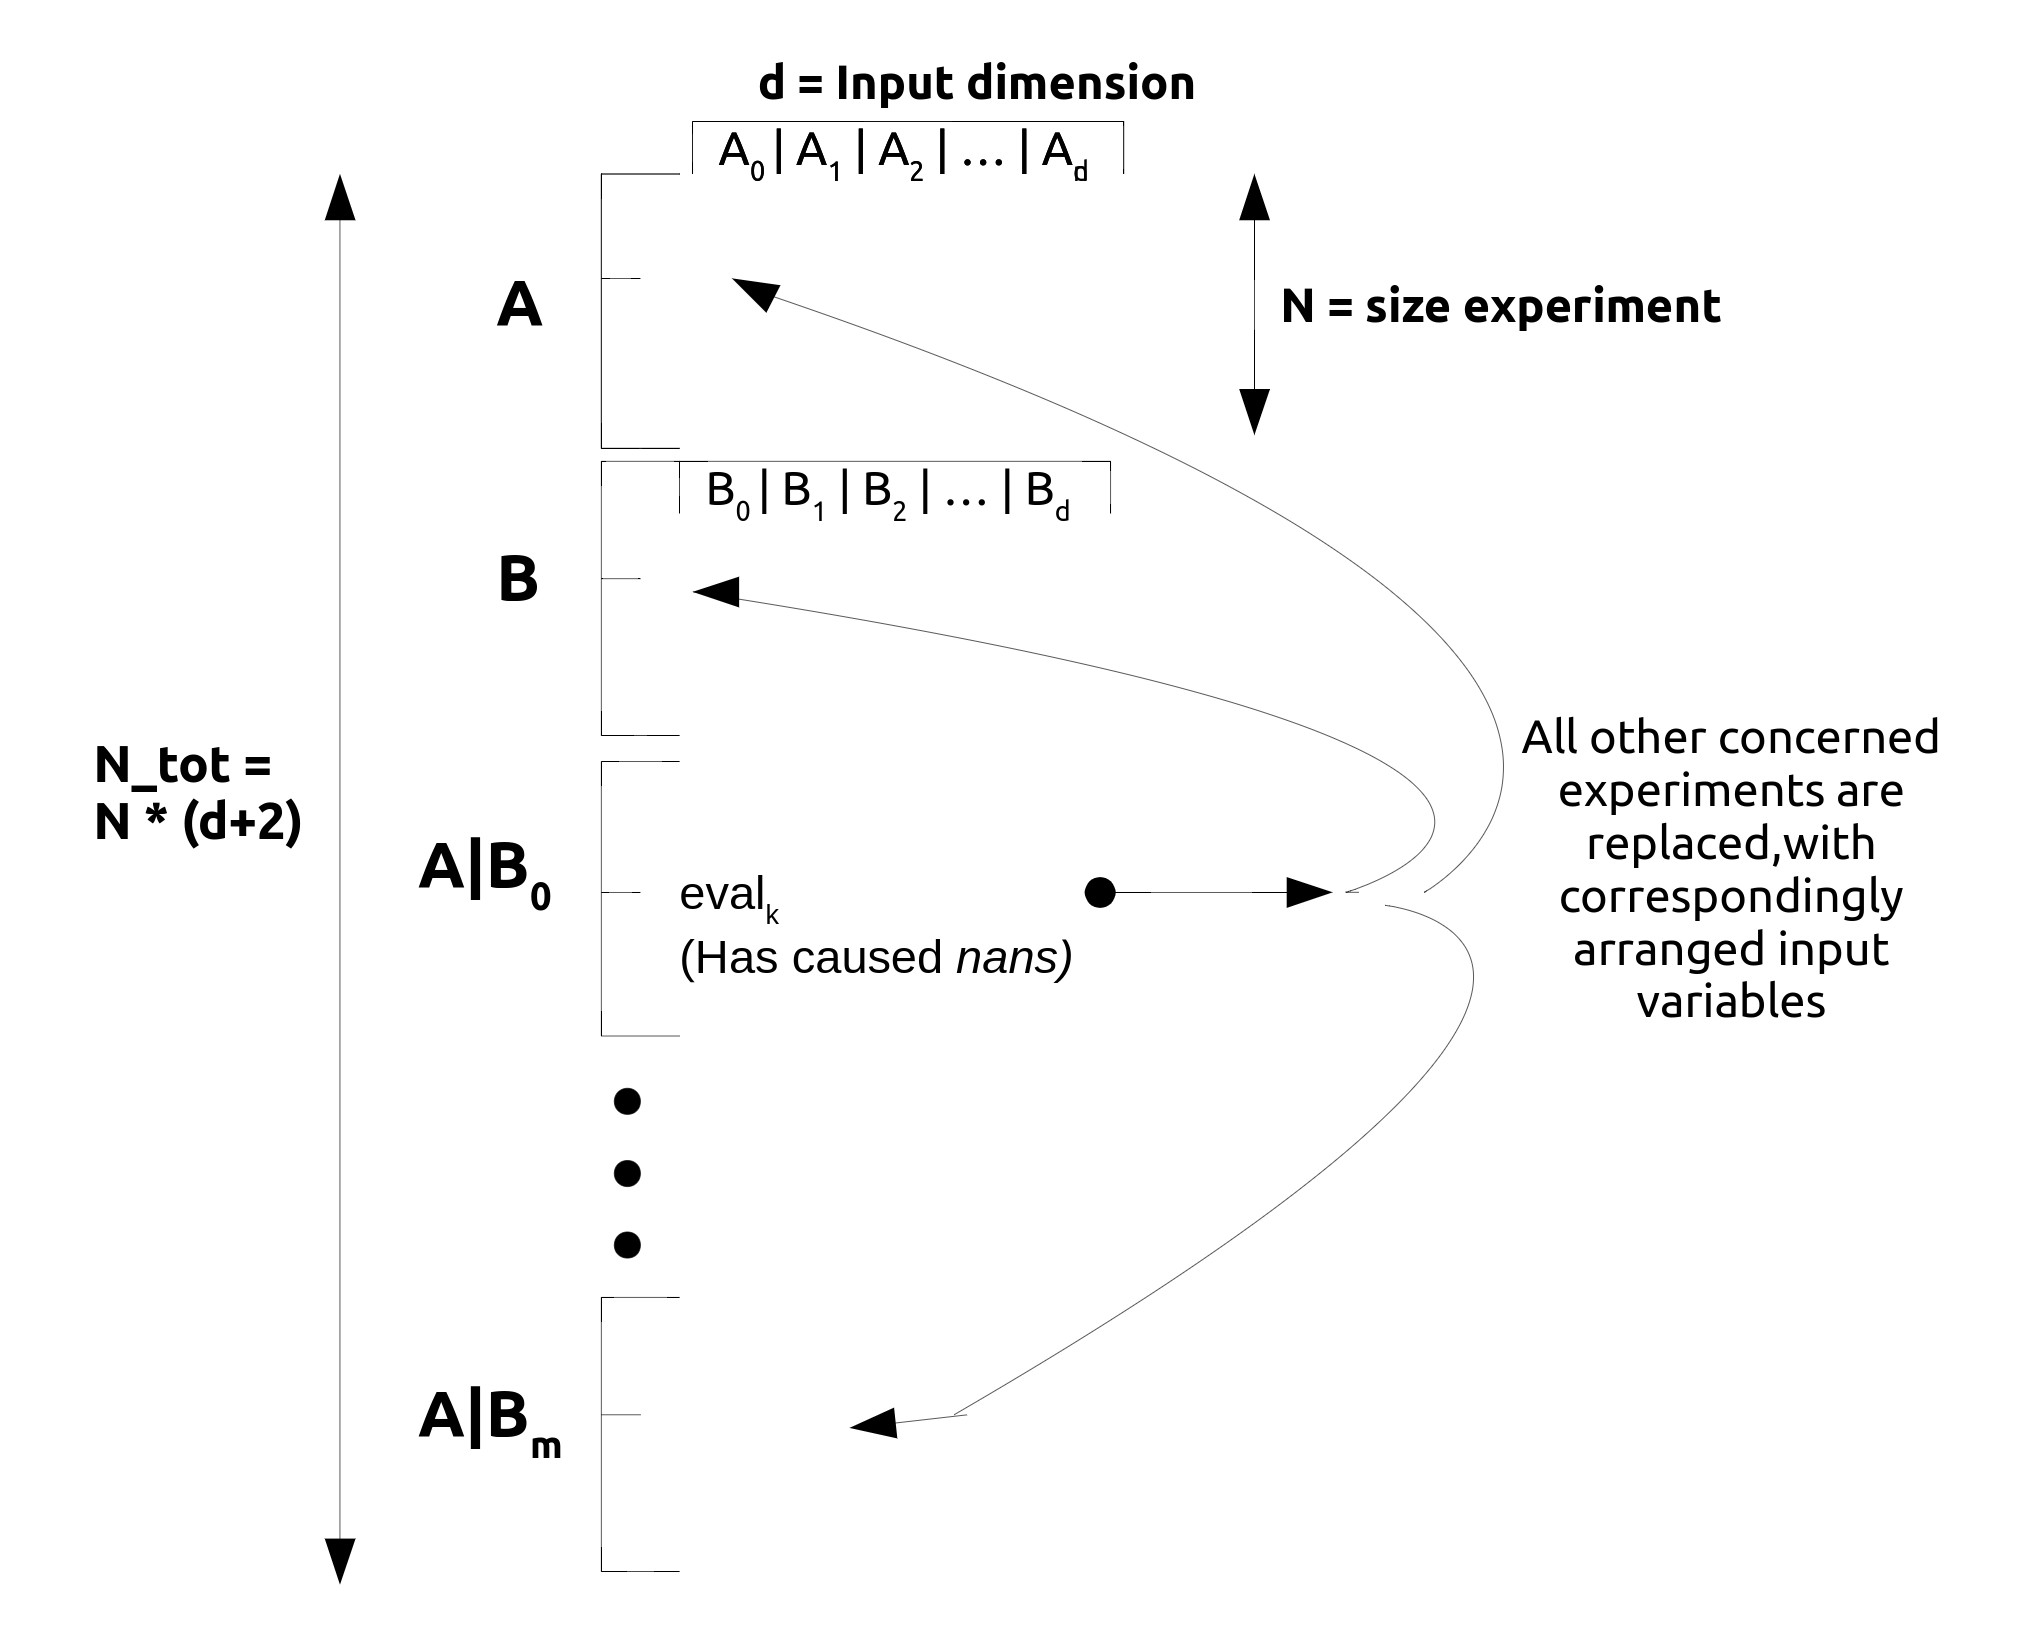
\includegraphics[scale=0.175]{schema_postprocessing.png}
      \caption{Organsiation des variables d'entrée, expliquant l'étape de postprocessing}
         \label{posprocessing}
\end{figure}


Une fois cette étape finie, on a accès aux indices de sobol pour chaque élément du champ. \\
Dans le cas de la poutre en flexion, prennant initialement 5 arguments en entrée (champ du module de young et champ du diamètre, densité, position de la force et norme de la force), la décomposition des deux champs en entrée fait que le modèle est ensuite régi par 24 variables aléatoires. Bien que cela fait augmenter la dimensionalité du problème, nous avons désormais la possiblité de travailler seuelement avec des variables aléatoires gaussiennes décorrélées, et donc faire une analyse de sensibilité classique.\\
La difficultée qui découle de cette analyse, est de trouver la manière qui permettra de relier les indices de sobol de ces variables aléatoire décorrélées, au champ stochastique d'origine. \\



\begin{figure}[H]
    \centering
    \begin{minipage}{0.45\textwidth}
        \centering
        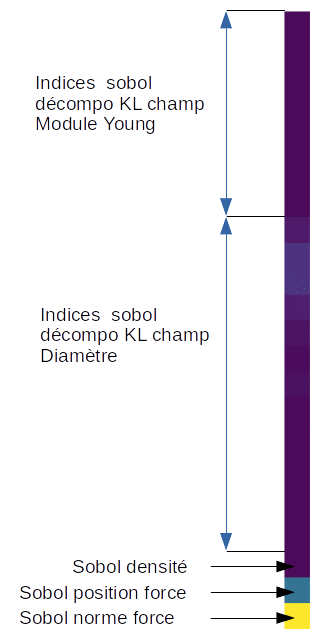
\includegraphics[height=1\textwidth]{sensitivity_rv_KL_anno.png} % first figure itself
        \caption{indices de sobol des V.A. de Karhunen-Loève pour la déflection maximale}
    \end{minipage}\hfill
    \begin{minipage}{0.45\textwidth}
        \centering
        
\includegraphics[width=1.35\textwidth]{sensitivity_field_KL.png} % second figure itself
        \caption{indices de sobol des V.A. de Karhunen-Loève pour le champ des contrainte de Von Mises}
    \end{minipage}
\end{figure}

Pour parvenir à faire ce lien, nous avions comme base différentes études sur le sujet, notamment le papier par \cite{Wei2017May}, sur l'analyse de sensibilité sur des modèles ayant des paramètres dépendants du temps. (Les variables étant gouvernées par le temps sont générallement stochastiques, ex: température, effort etc. ) \\

Mais ayant fait une analyse préliminaire de ces indices de sobol', des incohérences dans ces indices ont pu être remarqués. En effet, la somme de l'ensemble des indices du premier ordre doit être inferieure à 1 , et il ne peut y avoir d'indices négatifs. L'apparition d'indices de Sobol' négatifs peut être expliqué par un nombre d'experiences trop faible, nombre d'experiences qui lui même est limité par la mémoire disponible dans l'ordinateur. %Néanmoins, ce n'était pas la seule incohérence. Nous vous présentons ici les indices de Sobol' pour la contrainte de Von Mises dans chaque élément de la poutre, et nous essayons de voir l'influence de l'augmentation du nombre d'experiences sur le nombre d'indices de Sobol' qui sont négatifs, ou voir comment varie la somme de l'ensemble des indices de Sobol' associés à un seul élément. Nous utilisons ici $N=100 , N=500, N=1000, N=2500$



\subsubsection{Premiers essais d'analyse de la sensibilité du modèle }

Comme nous avions désormais accès aux différents indices de sobol de notre modèle basé sur la décompostion de Karhunen-Loève, le travail pouvait désormais se focaliser sur l'interprétation de ces différents indices. En effet, cette décomposition était très classique lors du travail avec des champs stochastiques, et plusieurs papiers de recherche se sont interessés à comment faire des  analyses de sensibilité de ce type de champs avec cette même décomposition. Comme mentionné précédemment, le travail de \cite{Wei2017May} offre une première approche pour l'interprétration de ces résultats, mais d'autres comme \cite{Pronzato2019Jul} ont aussi developpés des méthodes pour l'analyse de ces indices issus de l'expansion de Karhunen-Loève. 
Dans le travail de \cite{shangStochastic2013}, il est rapporté d'une méthodologie pour lier un modèle en élément finis d'Abaqus avec des champs stochastiques genérés avec MATLAB et pour l'analyse probabiliste de ce modèle. L'utilisation de l'expansion de KL y est aussi mentionné, et ce travail offre une analyse intéressante sur la capacité de cette méthode à reproduire le champs stochastique, en fonction de l'élément à partir duquel on troncature cette expansion. 

%\subsubsection{Essais sur la réponse du champs stochastique à la variation individuelle des variables auxilliaires issues de l'expansion de Karhunen-Loève}
%Comme dans les différentes méthodes proposées on génère le champ stochastique à partir d'une réalisation de variables auxilliaires et que l'on retrouve la corréspondance grâce aux vecteurs et valeurs propres de la matrice de covariance, il convient d'observer empiriquement sur un champ stochastique classique sa réaction face aux changement dans les différentes variables auxilliaires. Dans les notations adoptées précédemment, cela vient à vérifier l'amplitude et la nature du changement dans le champ stochastique $Y_{i}$, lors de changement dans les variables $\left(\xi_{i1}, \ldots, \xi_{iM_{i}}\right)$. \\

%Soit $Y_{i}$ un champ stochastique ayant comme modèle de covariance celui de Matern, et des  


\subsubsection{Interprétation et essais avec le papier : "Time-variant global reliability sensitivity analysis of structures with both input random variables and stochastic processes"}
Ce papier de recherche datant de 2017, offre une approche pour l'analyse de sensibilité de modèles définis dans le temps et leur analyse de fiabilité. En effet, de nombreuses structures mécaniques (ponts, tours etc.) sont soumis à des grandeurs variant dans le temps, et si celles se trouvent être continues dans celui ci, alors cette grandeur peut être représentée par un champ stochastique. Bien qu'il y aie une différence notable entre les grandeurs par rapport auxquelles il y a continuité (dans leur papier le temps, et nous l'espace), des analogies peuvent être faites. \\

L'approche se base sur la décomposition de Karhunen-Loève du champ stochastique, permettant de considérer le problème comme uniquement dépendant de variables aléatoire gaussiennes décorrélées, et de déduire la sensibilité du modèle au champ stochastique à partir de la sensibilité de chaque composant de la décomposition du champ. \\ 

La décomposition de KL est particulièrement utile pour le calcul de fonction d'enveloppe et les calculs fiabilistes. Dans ce papier, l'utilisation de l'experience de Monte-Carlo est essentiellement utilisée pour être comparée aux autres méthodes développées (\textbf{FOEF} : First Order Envelope Function et \textbf{AK-MCS} Active learning Kriging based Monte Carlo Simulation).\\

L'utilité de cette approche est de pouvoir identifier les sources principales d'incertitude ayant le plus d'influence sur la fiabilité du modèle. Enfin, elle permet de classer les variables selon leur ordre d'influence. \\

Néanmoins, leur approche se base sur la définition d'un état limite du modèle (par exemple la différence entre la contrainte maximale et la contrainte limite) et d'une fonction indicatrice de l'état limite, alors que nous cherchons à évaluer la sensibilité d'une grandeur en sortie (par exemple la contrainte) par rapport aux variables aléatoire en entrée. Ceci revient à priori à mesurer l'impact qu'à une variables en entrée sur la variance de la grandeur en sortie. \\

La définition mathématique de leur problème est la suivante : 

%Approximation de Kahrunen Loeve 
   \[
      \begin{array}{lp{0.8\linewidth}}
         S             & : Etat limite du modèle \\
         \textbf{X}    & : Vecteur de variables aléatoire \\
         \textbf{Y}(t) & : Vecteur de champs stochastiques dépendants du temps \\
         \textbf{Z}    & : Fonction de performance \\
         I_S 	       & : Fonction indicatrice \\
         R  		   & : Probabilité de défaillance sur l'intervalle [0,T]
      \end{array}
   \]
   \begin{eqnarray}   
S = \left\lbrace \left( \textbf{X},\textbf{Y}\right) :Z(t)=g\left(\textbf{X},\textbf{Y}(t),t\right)<0\ \forall t \in\left[0,T \right] \right\rbrace ;\\
I_S(t) = I_S(\textbf{X},\textbf{Y}(t),T) = 
\begin{cases}
	1 &  (\textbf{X},\textbf{Y}) \in S \\ 
	0 &  (\textbf{X},\textbf{Y}) \not\in S
\end{cases}\ ;\\
R = R(T) = P_r(I_S=1) = Pr(Z(t) = g(\textbf{X},\textbf{Y}(t) < 0, \forall t \in \left[0,T\right]) \ ;
   \end{eqnarray}\\

Les variables aléatoire et champs stochastiques ici définis sont tous indépendants entre eux. \\

Soient $\mu_{X}=(\mu_{X_{1}},\ldots,\mu_{X_{n}})$ et $\sigma_{X}=(\sigma_{X_{1}},\ldots,\sigma_{X_{n}})$ les vecteurs des moyennes et écarts types des variables aléatoires et $\mu_{Y}=(\mu_{Y_{1}},\ldots,\mu_{Y_{n}})$ et $\sigma_{Y}=(\sigma_{Y_{1}},\ldots,\sigma_{Y_{n}})$ les vecteurs des moyennes et écarts types des champs stochastiques. \\

Comme explicité lors de la définition de la décomposition de Karhunen-Loève, tout champ stochastique $Y_{i}(t)$ peut être écrit comme une somme de variables aléatoire gaussiennes décorrélées. 
\[
	\begin{array}{lp{0.8\linewidth}}
		Y_{i}(t)		& Approx. Procéssus Gaussien $Y_{i}$ \\
		\lambda_{ik}	& Valeur Propre de la matrice de covariance \\
		\xi_{ik}		& Variable Normale Centrée Réduite \\
		\varphi_{ik}(t)	& Vecteur propre de la matrice de covariance
	\end{array}
\]
   \begin{eqnarray}
Y_{i}(t) & = & \mu_{Y_{i}}(t) +  \sum_{k=1}^{M}\sqrt{\lambda_{ik}}\xi_{ik}\varphi_{ik}(t);
   \end{eqnarray}\\

D'où chaque champ gaussien peut être exprimé à partir d'un ensemble de variables aléatoire gaussiennes décorélées $\xi_{i}=(\xi_{i1},\ldots,\xi_{iM_{i}})$ et l'ensemble des champs est représenté par le vecteur $\xi=(\xi_{1},\ldots,\xi_{m})$. $\xi_{i}$ étant la représentation par des variables auxilliaires du champ $Y_{i}$. 

Grâce à la propriété de décomposition de la variance, on a :

\begin{figure}[H]
   \centering   
   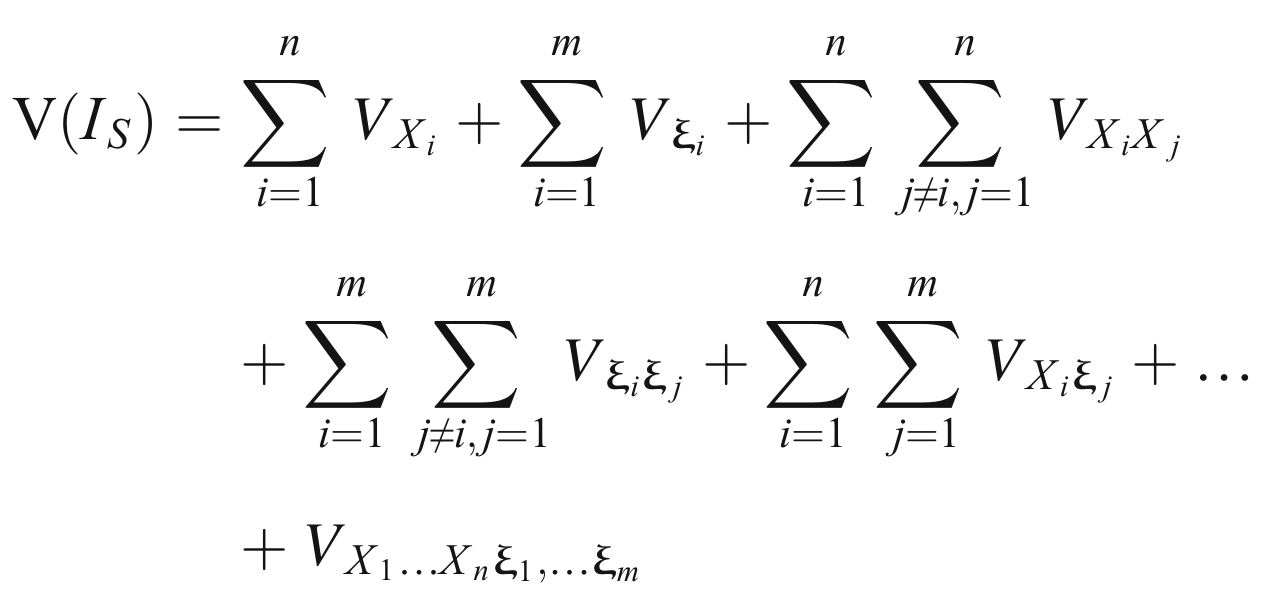
\includegraphics[scale=0.175]{DecompositionVariance.png}
      \caption{Decomposition de la variance de la fonction indicatrice}
         \label{VarDecompo}
\end{figure}

Ici, c'est la variance de la fonction indicatrice $I_{s}$ en sortie qui est traitée, mais ceci est faisable pour tout modèle dépendant d'un ensemble de variables aléatoire. Il est à remarquer ici que : 
$V_{X_{i}} = V\left[E\left(I_{S}|X_{i}\right)\right]$ qui est la variance conditionelle de la sortie $I_{S}$ lorsque la variable aléatoire $X_{i}$ est connue. \\ 
\\
Néanmoins, dans le cas du vecteur $\xi_{i} = (\xi_{i_{1}},\ldots,\xi_{i_{M_{i}}})$ on a: \\
\begin{eqnarray}
V_{\xi_{i}} = V\left[E\left(I_{S}|\xi_{i}\right)\right] = V\left[E\left(I_{S}|(\xi_{i_{1}},\ldots,\xi_{i_{M_{i}}})\right)\right] - \sum_{p=1}^{M_{i}}V_{\xi_{i_{p}}}
\end{eqnarray}
qui est la variance conditionelle de la sortie lorsque le vecteur aléatoire $\xi_{i}$ représentatif du champ stochastique $Y_{i}$ est connu.\\
\\  
Pour le calcul du vecteur des variances $V\left[E\left(I_{S}|(\xi_{i_{1}},\ldots,\xi_{i_{M_{i}}})\right)\right]$, dans le cadre d'une experience de Monte-Carlo, ceci pourrait se faire en rajoutant dans le plan d'experience, toutes les permutations associées à ces variables annexes aux champs stochastiques. \\

Avec le plan d'experience classique proposé par openTURNS, nous sommes en capacité de facilement calculer les indices de Sobol' du $1^{er}$ ordre de toutes les variables $S_{X_{i}}$ et $S_{\xi_{i_{p}}}$. Or nous cherchons $S_{\xi_{i}}$.\\
Dans le cas d'un modèle $F$, prenant en entrée un vecteur de champs stochastiques $Y = (Y_{1},\ldots,Y_{m})$ et un vecteur de variables aléatoires $X = (X_{1},\ldots,X_{n})$ et défini comme suit:  
\begin{align}
\omega = F(X,Y) &\  ,\omega \in \Re^{\aleph}
\end{align}


On peut définir une fonction $F^{'}$, utilisant la décomposition de Karhunen-Loève et seulement dépendante d'un ensemble de variables aléatoires décorrélées: 
\begin{align}
\omega = F^{'}(X,\xi) \\
\xi = (\xi_{1},\ldots,\xi_{m})\\
\xi_{i} = (\xi_{i_{1}},\ldots,\xi_{i_{M_{i}}})
\end{align} \\

Nous savons que : 
\begin{align}
V_{X_{i}} = V[E[\omega|X_{i}]] \\
S_{X_{i}} = \frac{V_{X_{i}}}{V(\omega)} \\
V_{X_{i}X_{j}} = V[E[\omega|X_{i}X_{j}]] - V_{X_{i}} - V_{X_{j}} \\
S_{X_{i}X_{j}} = \frac{1}{V(\omega)}V[E[\omega|X_{i}X_{j}]] - S_{X_{i}} - S_{X_{j}}
\end{align} \\

Néanmoins, à la différence des effets d'interactions et les sensibilités qui y sont associées, dans la cas de la sensibilité du champ stochastique, il semblerait qu'on ne soustraie pas l'effet de l'interaction du premier ordre, donc on n'aurait pas :
\begin{align}
S_{\xi_{i}} = S_{\xi_{i_{1}},\ldots,\xi_{i_{M_{i}}}} = \frac{1}{V(\omega)}V[E[\omega|\xi_{i_{1}},\ldots,\xi_{i_{M_{i}}}]] - \sum_{p=1}^{M_{i}}S_{\xi_{i_{p}}}
\end{align}

Mais plutôt seulement : 
\begin{align}
S_{\xi_{i}} = \frac{1}{V(\omega)}V[E[\omega|\xi_{i_{1}},\ldots,\xi_{i_{M_{i}}}]]
\end{align}

Ceci est intéressant dans la sens ou cela diminue grandement la complexité du calcul et qu'il ne faut plus que calculer les effets d'interaction et non plus les indices de sobol du premier ordre associés aux indices de KL des champs stochastiques. 

%Néanmoins dans le méthode présentée par \cite{Wei2017May}, on n'y fait pas mention d'une permutation de toutes les colonnes associées à un champ stochastique pour calculer l'effet d'interaction. Ceci fait supposer qu'il existe une autre manière d'arriver à trouver ces effet d'interaction, sans passer par cette permutation lors de l'experience de monte carlo ou que le calcul de cette interaction semblait trop triviale pour être mentionnée dans le papier:\\

%\begin{quote}
%\cite{Wei2017May}:\  By subtracting the first order partial variance $V_{X_{i}}$ and $V_{X_{j}}$ from $V[E(I_{S}|X_{i}, X_{j})]$, the second order partial variance $V_{X_{i}X_{j}}$ quantifies the second order interaction contribution between $X_{i}$ and $X_{j}$ to R. Similarly, $V_{\xi_{i}\xi_{j}}$ quantifies the second order interaction contribution between the stochastic process $Y_{i}(t)$ and $Y_{j}(t)$ to R, and $V_{X_{i}\xi_{j}}$ measures the second order interaction effect of the random variable $X_{i}$ and the stochastic process $Y_{j}(t)$ to R. \textbf{\textit{Higher order effect indices can be similarly defined and interpreted.}}
%\end{quote}

Le calcul à posteriori de ces interactions est possible, vu que nous n'avons qu'à comparer la moyenne des variance des deux échantillons de départ (\textbf{A} et \textbf{B}) à celle lorsque tout les paramètres du champs stochastique i sont connus ($V_{\xi_{i}}$). \\

Néanmoins, l'on ne peut pas inclure celles-ci dans le plan d'experience utilisé par openTURNS, vu que l'algorithme utilisé pour calculer les indices de Sobol' n'est concu que pour les calculs des indices de premier et second ordre de modèles gouvernés par un ensemble de variables aléatoires unitaires, et non des champs stochastiques. Pour parvenir à passer outre cette difficulté, un choix d'algorithme doit être fait pour le calcul de ces indices de sobol d'ordre fortement superieur. (Vu que pour les indices d'ordre 1, le choix de l'algorithme est entièrement libre.) Au vu du travail fait par PHIMECA sur l'analyse des lois asymptotiques des estimateurs des indices de Sobol \cite{dumas2017} ,l'on prendra comme estimateur celui de Martinez, mais il sera évidemment possible de rajouter à posteriori les autres estimateurs dans le workflow. \\ 

D'autre part, pour parvenir à garder cette complexité faible, nous sommes obligés de revoir la manière dont est fait le plan d'experience (la manière dont on mélange les différentes colonnes de nos deux samples \textbf{A} et \textbf{B}) puisque dans le cas de l'exemple de la poutre, nous aurions jusqu'a 5 fois moins de calculs à effectuer qu'en gardant tout les indices inutiles. \\
\begin{figure}[H]
   \centering   
   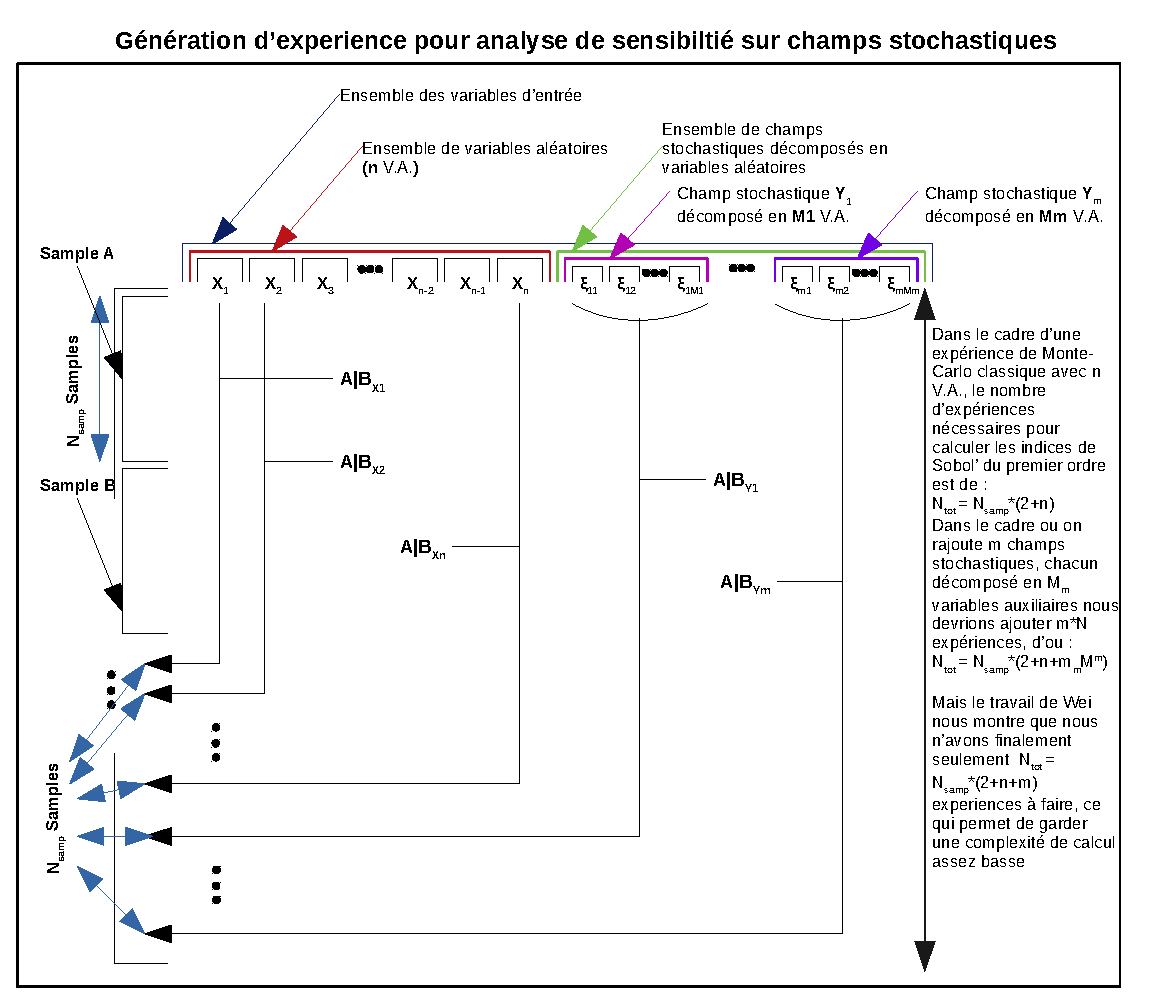
\includegraphics[scale=0.75]{Schema_Preparation_VA.pdf}
      \caption{Génération d’experience pour analyse de sensibiltié sur champs stochastiques}
         \label{expGenStoField}
\end{figure}
Les échantillons sont mélangés comme montré en figure \ref{expGenStoField}. 
Pour générer les samples de manière plus efficace, et être sur de couvrir l'ensemble du domaine de variance des lois d'entrée, est inclu dans le code la possibilité de générer l'échantillon en utlisant soit l'échantillonage LHS (Latin Hypercube Sampling), soit les séries à faible divergence (Low discrepancy series), soit une version optimisée du LHS (Simulated Annealing LHS). Bien sûr une génération entièrement aléatoire reste l'option de base.\\

\newpage
Pour le calcul formel de l'estimateur de Sobol', nous allons utilisons la méthode par Saltelli, détaillée dans le papier par \cite{dumas2017}. Ce papier détail aussi la manière de calculer l'erreur dans le calcul de l'estimateur, valeur importante pour connaître la pertinence de l'estimateur. 

Détail du calcul de l'indice de Sobol' :

   \[
      \begin{array}{lp{0.8\linewidth}}
        \prescript{c}{}{\mathbf{Y}}^{A}   & : Sortie du modèle associé à l'echantillon A du plan d'experience \\
        \prescript{c}{}{\mathbf{Y}}^{B}   & : Sortie du modèle associé à l'echantillon B du plan d'experience \\
        \prescript{c}{}{\mathbf{Y}}^{E}   & : Sortie du modèle associé à l'echantillon issu de A ou l'on a inseré une partie de B \\
         \mathbf{S} 					  & : Indice de Sobol' \\
      \end{array}
   \]\\
\* Les échantillons centrées sont annotés du prescript c \*

   \begin{gather}   
S = \frac{Cov\left[\prescript{c}{}{Y}^{B},\prescript{c}{}{Y}^{E}\right]}{Var\left[\prescript{c}{}{Y}^{A}\right]} \\
= \frac{\frac{1}{n}\Sigma_{k=0}^{n}\prescript{c}{}{Y}^{B}\prescript{c}{}{Y}^{E} - \left(\frac{1}{n}\Sigma_{k=1}^{n}\prescript{c}{}{Y}^{B}\right)\left(\frac{1}{n}\Sigma_{k=1}^{n}\prescript{c}{}{Y}^{A}\right)}{\frac{1}{n}\Sigma_{k=0}^{n}(\prescript{c}{}{Y}^{B})^{2}-(\frac{1}{n}\Sigma_{k=0}^{n}\prescript{c}{}{Y}^{B})^{2}}
   \end{gather}\\
   
Comme les échantillons sont centrées par rapport à leurs moyennes respectives, le numérateur et le dénominateur se simplifient et on obtient l’estimateur suivant :

	\begin{equation}
		S = \frac{\frac{1}{n}\Sigma_{k=0}^{n}\prescript{c}{}{Y}^{B}\prescript{c}{}{Y}^{E}}{\frac{1}{n}\Sigma_{k=0}^{n}\left(\prescript{c}{}{Y}^{A}\right)^{2}}
	\end{equation}


Avec l'échantillonnage présenté précédemment, le calcul de l'estimateur de Sobol se fait très directemement avec la formule de Saltelli, même lorsque la dimension de la sortie est plus grande que 1.

Pour pouvoir justifier de la pertinence de l'estimateur, on calcule l'intervalle de confiance à 0.975, qui permet de montrer la précision de l'estimateur et de nuancer son analyse. Pour le calcul de cet intervalle de confiance, on utilise la méthode Delta, méthode utilisée par Jansen \textit{et al} (2014) ou de même par \cite{dumas2017}. Le détail de cette méthode est donné ci dessous.

On pose suite à l’équation simplifiée précédente :

\begin{equation}
U_{i} = \left(\prescript{c}{}{Y}^{B}\prescript{c}{}{Y}^{E},\left(\prescript{c}{}{Y}^{A}\right)^{2}\right)^{T} \\
\end{equation} \\
  
Ensuite l'on défini :
\begin{equation}
\Psi_{S}(x,y) = \frac{x}{y} \\
\end{equation} \\

Ceci implique :
\begin{equation}
S_{N} = \Psi_{S}\left(\overline{U}_{N}\right)
\end{equation} \\

Grâce au théorème central limite:
\begin{equation}
\sqrt[]{N}\left(\overline{U}_{N}-\mu\right)\xrightarrow[N\to\infty]{\mathcal{L}}\mathcal{N}_{2}\left(0,\Gamma\right) 
\end{equation}\\

Ou $\Gamma$ est la matrice de covariance de $U_{1}$ et :
\begin{equation}
\mu=
\begin{cases}
	Cov\left[Y^{B},Y^{E}\right] \\
	Var\left[Y^{A}\right]       \\
\end{cases}\\
\end{equation}

De l'utilisation de la méthode delta : 
\begin{equation}
\sqrt[•]{N}\left(S_{N}-S\right)\xrightarrow[N\to\infty]{\mathcal{L}}\mathcal{N}_{1}\left(0,g^{T}\Gamma g\right)
\end{equation}
ou $g=\nabla\Psi_{S}(\mu)$.\\ 

Finalement, pour tout x,y tel que $y \neq 0$ :
\begin{equation}
\nabla\Psi_{S}(x,y)=\left(\frac{1}{y},\frac{-x}{y^{2}}\right)^{T}
\end{equation}

La matrice de covariance $\Gamma$, tout comme le vecteur $g$ se calculent bien analytiquement dans le cas de l'indicateur de Saltelli', néanmoins le calcul du gradient peut très bien se faire informatiquement, notamment dans le cas d'estimateurs plus complexes.

Pour recupérer l'intervalle de confiance de l'estimateur nous utilisons le quantile de la loi normale centrée réduite à 97.5\%, multiplié par la racine de la variance calculée précédemment. 

Finalement, l'on récupère les indices de Sobol' pour les différents élements de la poutre tout comme leur intervalle de confiance: 



\begin{figure}[H]
   \centering   
   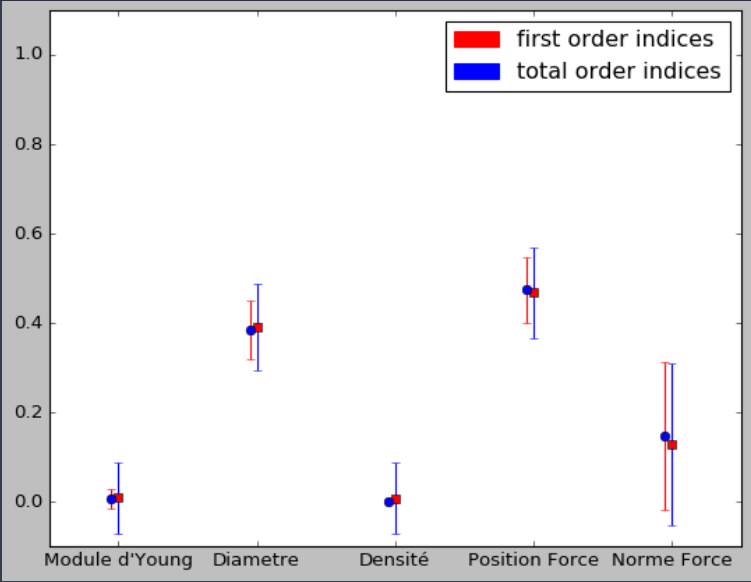
\includegraphics[scale=0.195]{sensibiliteDeflection10K.png}
      \caption{Sensibilité de la déflection maximale aux champs et variables d'entrée.}
         \label{MaxDeflec}
\end{figure}

\begin{figure}[H]
   \centering   
   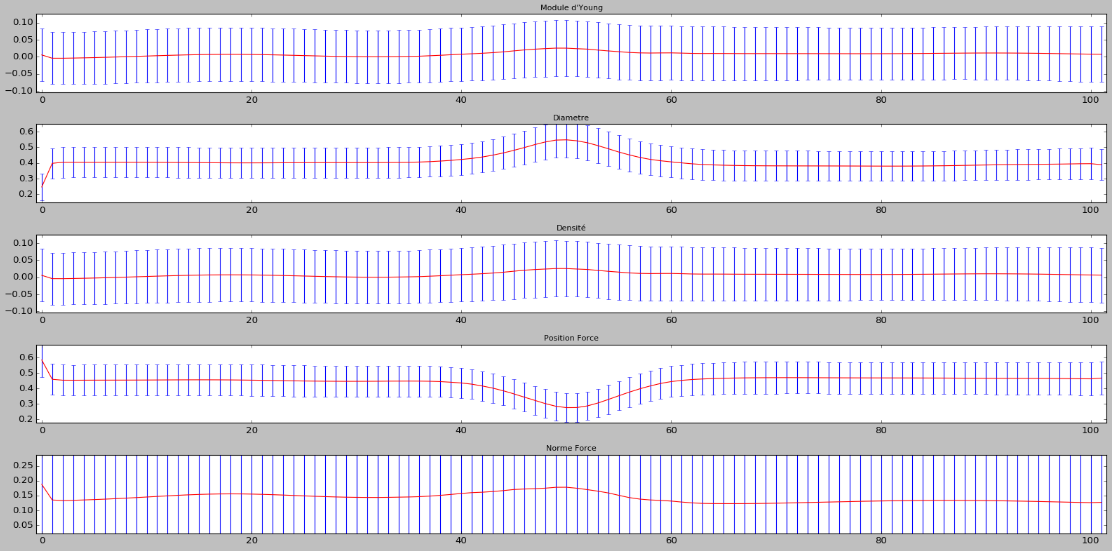
\includegraphics[scale=0.255]{sensibiliteVonMises10K.png}
      \caption{Sensibilité de la contrainte de Von-Mises aux champs (Module d'Young, diamètre) et variables d'entrée.(densité, position, Norme de la force
      )}
         \label{MaxDeflec}
\end{figure}
L'on peut voir qu'il y a très peu d'écarts entre les indices d'ordre total et premier ordre. Les effets d'interaction sont donc très peu présents entre les variables d'entrée.\\
\\
Finalement une comparaison entre un exemple de la documentation d'\textit{openTURNS} et les codes développés durant ce stage peut être faite, pour confirmer que les méthodes implémentées sont exemptes d'erreurs. 

\begin{figure}[H]
   \centering   
   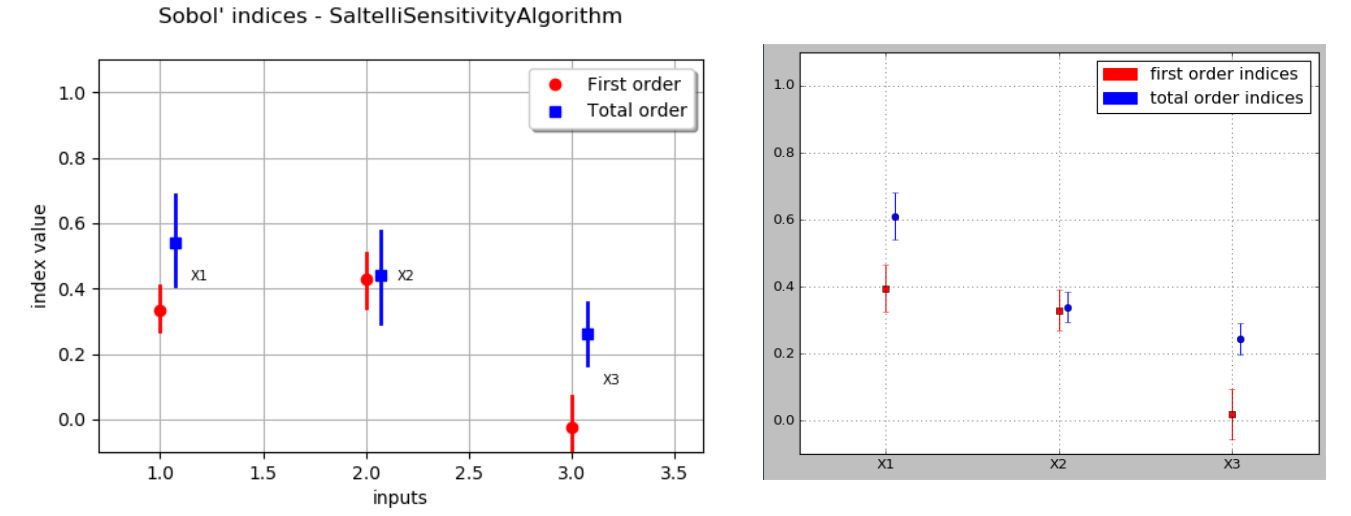
\includegraphics[scale=0.255]{comparisonOtMe.png}
      \caption{Comparaison entre la solution par openturns (à gauche) et la notre (à droite), pour un échantillon de taille 1000 sur la fonction d'Ishigami}
         \label{Comparison}
\end{figure}

L'on observe, que pour cet échantillon de 1000, l'indice de Sobol' calculé avec nos codes est relativement proche de ceux calculés avec \textit{openTURNS}, même si des écarts subsistent, notamment au niveau de la variance. Cette variance s'explique en partie par l'incertitude dans les variables d'entrées (tout échantillon de 1000 est à priori unique).

Les codes ayant montré leur utilisabilité, il était enfin possible d'essayer d'appliquer cette méthodologie à un système plus complexe, un échangeur de chaleur air-air modelisé avec NASTRAN. 
 
\subsection{Application au modèle NASTRAN d'échangeur thermique}
\subsubsection{Définition et analyse de la problématique}

Comme nous l'avions mentionné avant, la finalité de ce travail de quasi-recherche et développement de codes, était de parvenir à induire des défauts stochastiques dans un modèle numérique, et de mesurer la sensibilité de ce modèle à ces perturbations. 

Le modèle en question est celui d'un échangeur thermique d'utilisation aéronautique. Cette pièce doit être  capable de supporter et échanger la température de deux flux d'air perpendiculaires, l'un à la température de l'air en haute altitude - jusqu'à -50\degree - et l'autre aux températures moteurs allant jusqu'à 600C. \\

\begin{figure}[H]
   \centering   
   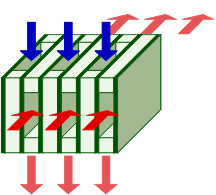
\includegraphics[scale=0.5]{principeEchangeur.png}
      \caption{Principe de l'échangeur à chaleur air-air}
         \label{principleExchanger}
\end{figure}

Ce projet est financé par l'union européenne, et la fabrication est assurée par le fabricant allemand \textbf{LIEBHERR}. Ce dernier sous-traite certaines étapes de l'étude, comme les essais physiques sur des échantillons de l'échangeur, tâche réalisée par \textbf{Lortek}, la construction d'un modèle paramétrique numérique de l'échangeur, tâche réalisée par \textbf{Epsilon}, et enfin la partie analyse de sensibilité et déformation moteur réalisée par \textbf{Phimeca}. \\

Ce projet à donc impliqué l'étroite collaboration de ces différents acteurs, vu que pour l'analyse de sensibilité il nous fallait utiliser le modèle contruit par \textbf{Epsilon}, et introduire des incertitudes dans les paramètres, dont la nature et les paramètres ont été récupérées dans les mesures faites par \textbf{Lortek}.


\begin{figure}[H]
   \centering   
   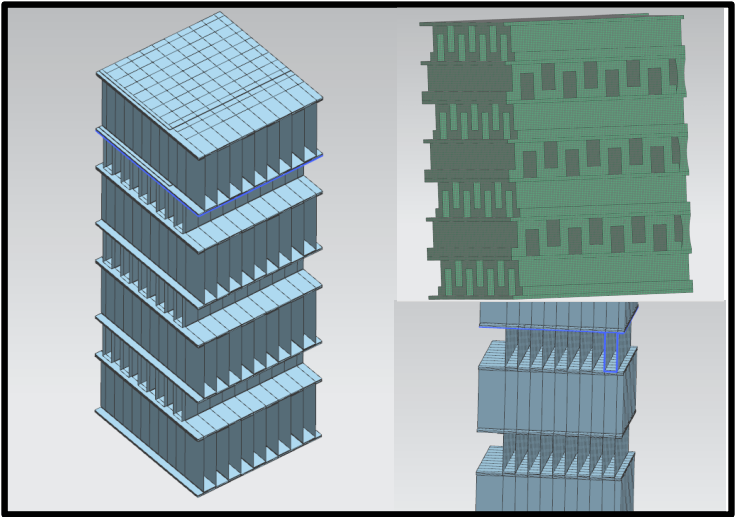
\includegraphics[scale=0.3]{exchangerModel.png}
      \caption{Modèle Nastran de l'echangeur de chaleur - Siemens Simcenter 3D}
         \label{exchangerModel}
\end{figure}

Pour bien se coordoner sur le projet, des réunions se sont régulièrement tenues, permettant de se tenir à jour sur les avancements de chacun, et de définir les prochaines étapes à atteindre. \\ 

Dans le cas de l'étude à réaliser par \textbf{Phimeca}, le sujet d'analyse était l'étude de l'influence de la variabilité dans les paramètres des aillettes de l'échangeur de chaleur sur la localisation de la défaillance. Dans le cas de l'échangeur de chaleur, la défaillance correspond à une rupture d'aillette, ou une perte d'étancheité. \\

Numériquement, la rupture se traduit par une contrainte maximale supérieure à la contrainte maximale suportée par le matérieau constituant de la pièce. L'analyse de la pièce se traduit donc par l'étude de l'effet de la maitrise des paramètres de l'ailette (épaisseur, planéitée, angle...) sur la localisation de la contrainte maximale. 

\begin{figure}[H]
   \centering   
   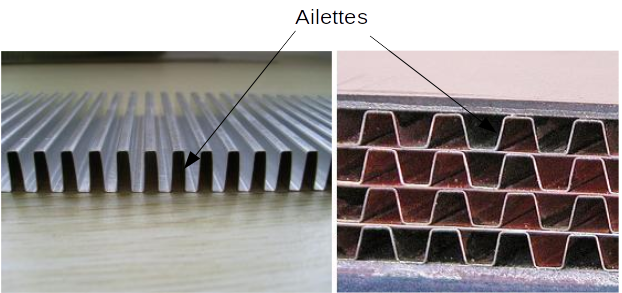
\includegraphics[scale=0.45]{SchemaAilettes.png}
      \caption{Ailettes d'un échangeur de chaleur}
         \label{SchemaAilettes}
\end{figure}

\subsubsection{Mise en place de méthodologie }

Pour parvenir à introduire ces variabilités différentes approches et modèles de champs stochastiques peuvent être prises en considération, puisque les réalisations peuvent fortement varier en fonction des paramètres et modèles. Il est en outre difficile de générer un champ qui serait indépendant du maillage sur lequel il est réalisé, ou du moins qui ressemblerait à un échantillon d'un champ plus grand. 


\begin{figure}[H]
   \centering   
   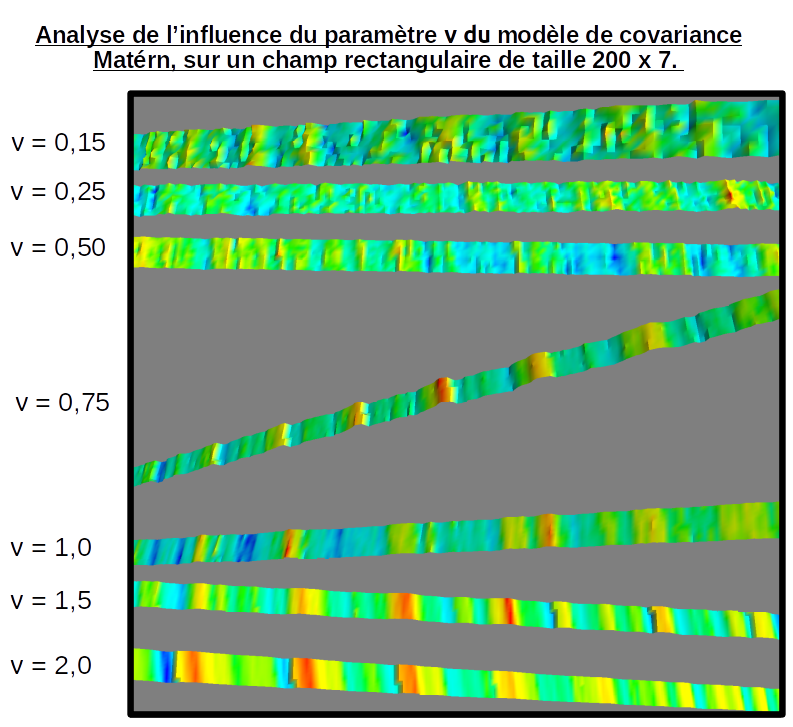
\includegraphics[scale=0.3]{maternNu.png}
      \caption{Impacte d'un paramètre sur, un champ}
         \label{maternNu}
\end{figure}

En deux dimensions, un champ stochastique peut être vu comme un maillage uniforme, ou une valeur est associée à chaque noeud, et ou la valeur à chaque noeud est corrélée à la distance et valeur des nœuds proches. La première idée aurait donc été d'appliquer directement une déformation générée par un champ de la même taille que le maillage d'une ailette aux nœuds constituant l'ailette, et donc de simuler une déformation stochastique par ailette, mais en écartant du coup toute corrélation inter-ailettes.
La déformation se serait fait par translation de chaque nœud suivant l'axe normal au plan de l'ailette.
Cette méthode a vite été écartée, puisque la génération de champs sur des maillages sous forme de long rectangle étiré était bien moins précise et contrôlables, allant jusqu'à des réalisation quasi constantes ou périodiques. De plus le nombre de champs généré par passe serait très important, alors qu'il serait plus simple de ne  génerer qu'un seul champ par plaque et de paramétriser les déformations.\\

D'après le travail réalisé par \cite{Goka2019Jun}, une méthodologie pour modéliser au mieux les imperfections de conception d'une pièce et se rapprocher de défauts réalistes existe. 
Dans son travail de thèse, \cite{Goka2019Jun} analyse les différentes manières de représenter les défauts de forme d'une pièce issues des imperfections de fabrication. Chaque méthode qu'elle soit paramétrique (Courbes de Bézier, B-Spline, NURBS), aléatoire (Bruit Gaussien), issue de morphing, d'un Skin-Model ou encore basé sur des modes (FFT, Polynômes, PCA, Décomposition modale métrique, champs aléatoires... ) est analysée et jugée par rapport à 4 critères : 
\begin{itemize}
	\item capacité à représenter les défauts de forme et les ondulations
	\item compatibilité avec une représentation probabiliste du champ des défauts <=> amplitude des défauts de méthode doivent être modélisées par des lois de probabilité.
	\item compatibilité avec les méthodes d'analyse probabiliste existantes, et interprétabilité physique (les coefficients contrôlant l'amplitude des défauts et leur distribution doivent représenter une grandeur physique mesurable) . 
	\item doit être capable de modéliser des contacts locaux entre pièces et de retrouver les points de contact 
\end{itemize}

L'applicabilité de ces méthodes a notre problème dépend aussi de la réponse à ces critères, et elles ont étés développées au cours de cette thèse en vue de leur utilisation sur des projets d'analyse comme celui-ci. 
La méthode retenue par Goka au cours de son analyse est la méthode de la décomposition métrique modale. 
Cette méthode ne s'appuie ni sur des équations du mouvement de la mécanique vibratoire, ni sur la méthode des éléments finis. Elle permet d'introduire des défauts dans un modèle en appliquant une translation à chaque noeud du maillage de la surface. Cette translation est appliquée à l'aide de ce qu'on appelle les vécteurs modaux. 
Ces vecteurs modaux représentent un défaut élémentaire de la surface. Il existe différent types de déformations élémentaires, et chacun d'eux est à rapporter avec une forme élémentaire. De même ces vecteurs modaux sont généralement représentés dans la base qui est la plus adaptée pour représenter la pièce à laquelle on applique ces défauts. Par exemple les défauts élémentaires d'une surface plane cylindrique. 

\begin{figure}[H]
   \centering   
   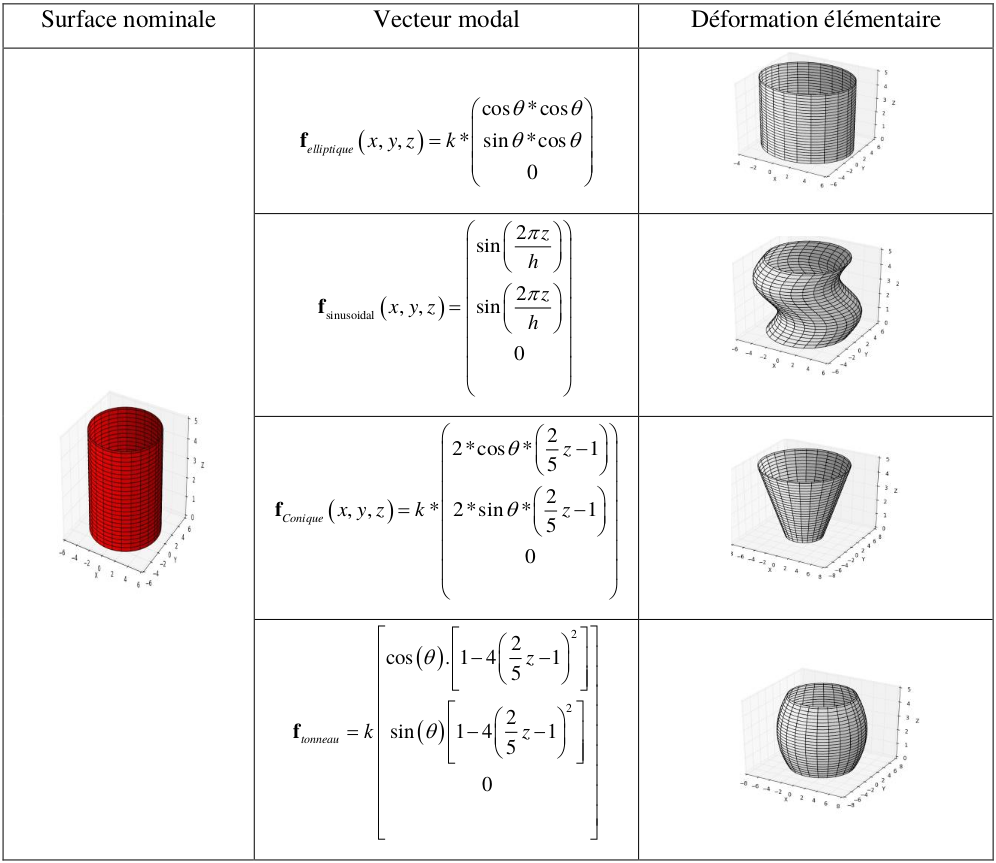
\includegraphics[scale=0.3]{VecteurModalCylindre.png}
      \caption{Vecteur des déformations modales pour un cylindre}
         \label{VecteurModalCylindre}
\end{figure}

Analytiquement, un champ modal est défini de la manière suivante (en coordonnées cartésiennes ici):

\begin{equation}
\textbf{f}(x,y,z) = 
\begin{bmatrix}
\textbf{f}_{x}(x,y,z) \\
\textbf{f}_{y}(x,y,z) \\
\textbf{f}_{z}(x,y,z)
\end{bmatrix}_{(x,y,z)}
\end{equation} 

ce vecteur f(x,y,z) est appliqué à chaque point de la surface de la pièce que l'on souhaite déformer. Le champ modale représente les défauts de forme de la surface, ou encore l'écart entre les positions théoriques parfaites et les positions réelles des points. 

On peut écrire que pour chaque point de la surface nominale $ M_{n}(x_{n}, y_{n}, z_{n}) $ on applique ce vecteur $ f(x,y,z) $ pour obtenir un nouveau point $ M_{f}(x_{f}, y_{f}, z_{f}) $ :
\begin{equation}
\begin{pmatrix}
x_{f} \\
y_{f} \\
z_{f} 
\end{pmatrix} = 
\begin{pmatrix}
x_{n} \\
y_{n} \\
z_{n} 
\end{pmatrix} +
\begin{pmatrix}
\textbf{f}_{x}(x_{n},y_{n},z_{n}) \\
\textbf{f}_{y}(x_{n},y_{n},z_{n}) \\
\textbf{f}_{z}(x_{n},y_{n},z_{n})
\end{pmatrix}_{(x,y,z)}
\end{equation}

Le champ modal total représentant les défauts de forme de la surface est défini par la somme pondérée des modes élémentaires appliqués à chaque nœud de la surface :

\begin{equation}
\textbf{f}_{pa,A_{0}} = 
\begin{pmatrix}
\textbf{f}_{xpa,A_{0}} \\
\textbf{f}_{ypa,A_{0}} \\
\textbf{f}_{zpa,A_{0}} 
\end{pmatrix}_{(x,y,z)} = 
\sum_{j=1}^{n}\lambda_{pa,j}\times\textbf{f}_{pa,j,A_{0}}
\end{equation} \\


Ici, $ \textbf{f}_{pa,A_{0}} $ est le champ modal total de la surface \textit{a} de la pièce \textit{p} et exprimé au point $ \textit{A}_{0} $ ; \ $ \textbf{f}_{pa,j,A_{0}} $ est le vecteur modal correspondant au $j^{ème}$ défaut de forme élémentaire écrit en un point $\textit{A}_{0}$ de la surface \textit{a} de la pièce \textit{p} ; \ $\lambda_{pa,j}$ représente le coefficient d'amplitude du $j^{ème}$ défaut de forme élémentaire de la surface a de la pièce p. Les vecteurs modaux dépendent de la classe et géométrie de la surface, tout comme du moyen de fabrication utilisé. \\ 


Les vecteurs modaux sont ensuite normés, pour que les coefficient d'amplitude $\lambda_{pa,j}$ représentent bien une grandeur physique mesurable (métrique).\\
Le calcul de la norme se limite à calculer la norme maximale du champ vectoriel modal pour tout les points de la surface, avant de normer ce maximum à 1mm : 

\begin{equation}
max(\Vert\textbf{f},(M)\Vert)_{1\leq j\leq n} = 1[mm]
\end{equation}\\

L'on obtient les différents modes en étudiant les caractéristiques intrinsèques et les degrés d'invariance de la surface nominale. Quatre types de modes peuvent être distingués : 
\begin{itemize}
	\item Les modes rigides qui ne changent pas la nature de la surface: les modes de translation et de rotation de la surface correspondent au premier modes. 
	\item Les modes dis de "dilatation" qui correspondent à des variations des caractéristiques de la surface. 
	\item Les modes d'ondulation définis pas des déviations sinusoidales le long des \textit{Eléments Géométriques de Reférence Minimum}\footnote{Les éléments géométriques de référence sont des formes géométriques (plans, cylindre, axe) parfaites qui servent de base pour mesurer les écarts. Dans le cas du modèle de l'échangeur de chaleur, ces plans de référence sont les plans d'origine.}(EGRM) de la surface.  
	\item Les modes des section définissant des variations de caractéristiques intrinsèques en utilisant des coordonnées polaires(\textit{Ref?}). Ces modes font varier le profil ou la géormétrie de la section droite d'une surface. Dans le cas d'une ailette d'une passe de l'échangeur, ce la revient à faire varier le profil de l'ailette en fonction de la direction du flux d'air. Ceci donne à l'ailette une sorte de géométrie de "ruban". 
	\item Les modes quelconques sont ceux n'appartenant pas aux autres catégories. 
\end{itemize} \

Le choix final des modes de déformation se fait finalement à partir des données issues d’expériences ou connaissances en fabrication. En fonction du procédé de fabrication certains défauts sont en effet récurrents. L'amplitude des défauts est déterminée grâce à des mesures prises sur les pièces fabriquées. 
\linebreak

Le choix de cette méthode semblait donc très adapté, puisque l'utilisation de défauts paramétrisés permet de facilement contrôler des défauts complexes avec qu'un seul paramètre, et évite de devoir générer un grand nombre de déformations stochastiques qui sont bien moins contrôlables et plus coûteuses en temps de calcul à générer. 
De plus l'utilisation de cette méthode permet de garder une grande maîtrise des défauts et des corrélations inter-défaut.
\linebreak

En tant qu'illustration, un schéma détaillant la méthode pour la déformation d'une passe de l'échangeur de chaleur avec la méthode de la déformation modale métrique est donné ci dessous. Sur ce schéma, le coefficient d'amplitude $\lambda_{pa,j}$ est donné par un champ stochastique défini sur un maillage de la même taille que la passe, et l'élément géométrique minimal est l'ensemble d’arêtes perpendiculaires aux deux flux d'air.\\ 
La valeur du champ stochastique en un point donne l'écart maximal entre la surface nominale et la surface "réelle" , et la déformation en elle même suit un polynôme du second ordre s'annulant aux bornes inférieures et supérieures de la passe. 


\begin{figure}[H]
   \centering   
   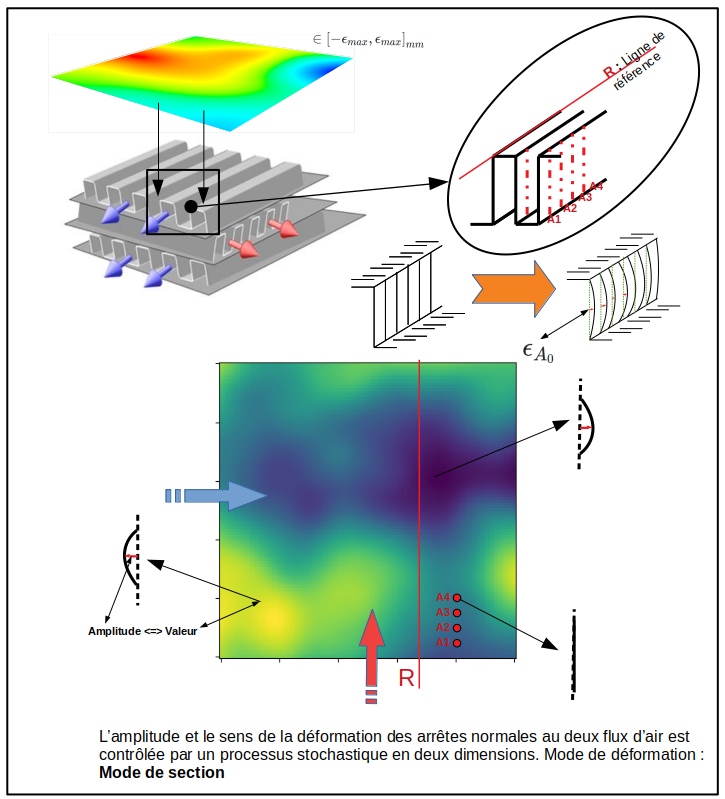
\includegraphics[scale=0.45]{SchemaModesDeformation.png}
      \caption{Schema de l'influence entre la réalisation d'un champ stochastique et la déformation modale de la passe de l'échangeur}
         \label{SchemaModesDeformation}
\end{figure}

Cette méthode était hautement fonctionnelle, car les déformations sont toutes corrélées au sein d'une même passe, avec même la possibilité de parvenir à une corrélation tri-dimensionnelle, si l'on génère un champ 3D . 

\subsubsection{Application de la méthode de la déformation modale métrique pilotée par champ stochastique sur un modèle Simcenter 3D Nastran}

Bien sûr, bien que théoriquement simple, l'implémentation de cette méthode au sein de Simcenter NX Nastran était plus complexe, car l'on devait pouvoir garder le contrôle total sur la géométrie nominale de la pièce - peu importe quels paramètres géométriques originaux on imposait - et aussi un contrôle total sur quel types de passes/ plaques de séparation on introduisait des défauts, et enfin un contrôle total sur les processus stochastiques, leurs fonctions de covariance, et bien sûr les modes de déformation modale et leur nombre.\\

Néanmoins plusieurs difficultés ont été rencontrées lors de l'écriture des codes, puisque les scripts python devaient interagir avec le logiciel de Siemens. Simcenter NX possède un langage de "scripting" appelé NX, qui permet d'utiliser les fonctions de Simcenter depuis un interpréteur et d'automatiser des tâches dans ce qu'on appelle des journaux. L'accès au capacités de scripting de Simcenter peut se faire à partir de différents langages, dont le Visual Basic ou Python, bien que très peu de tutoriels existent pour Python. \\

Mais c'est bien le Python qui a été choisi au final de par sa plus grande simplicité par rapport au Visual Basic et l'existence d'une documentation fournie. \\

\begin{figure}[H]
   \centering   
   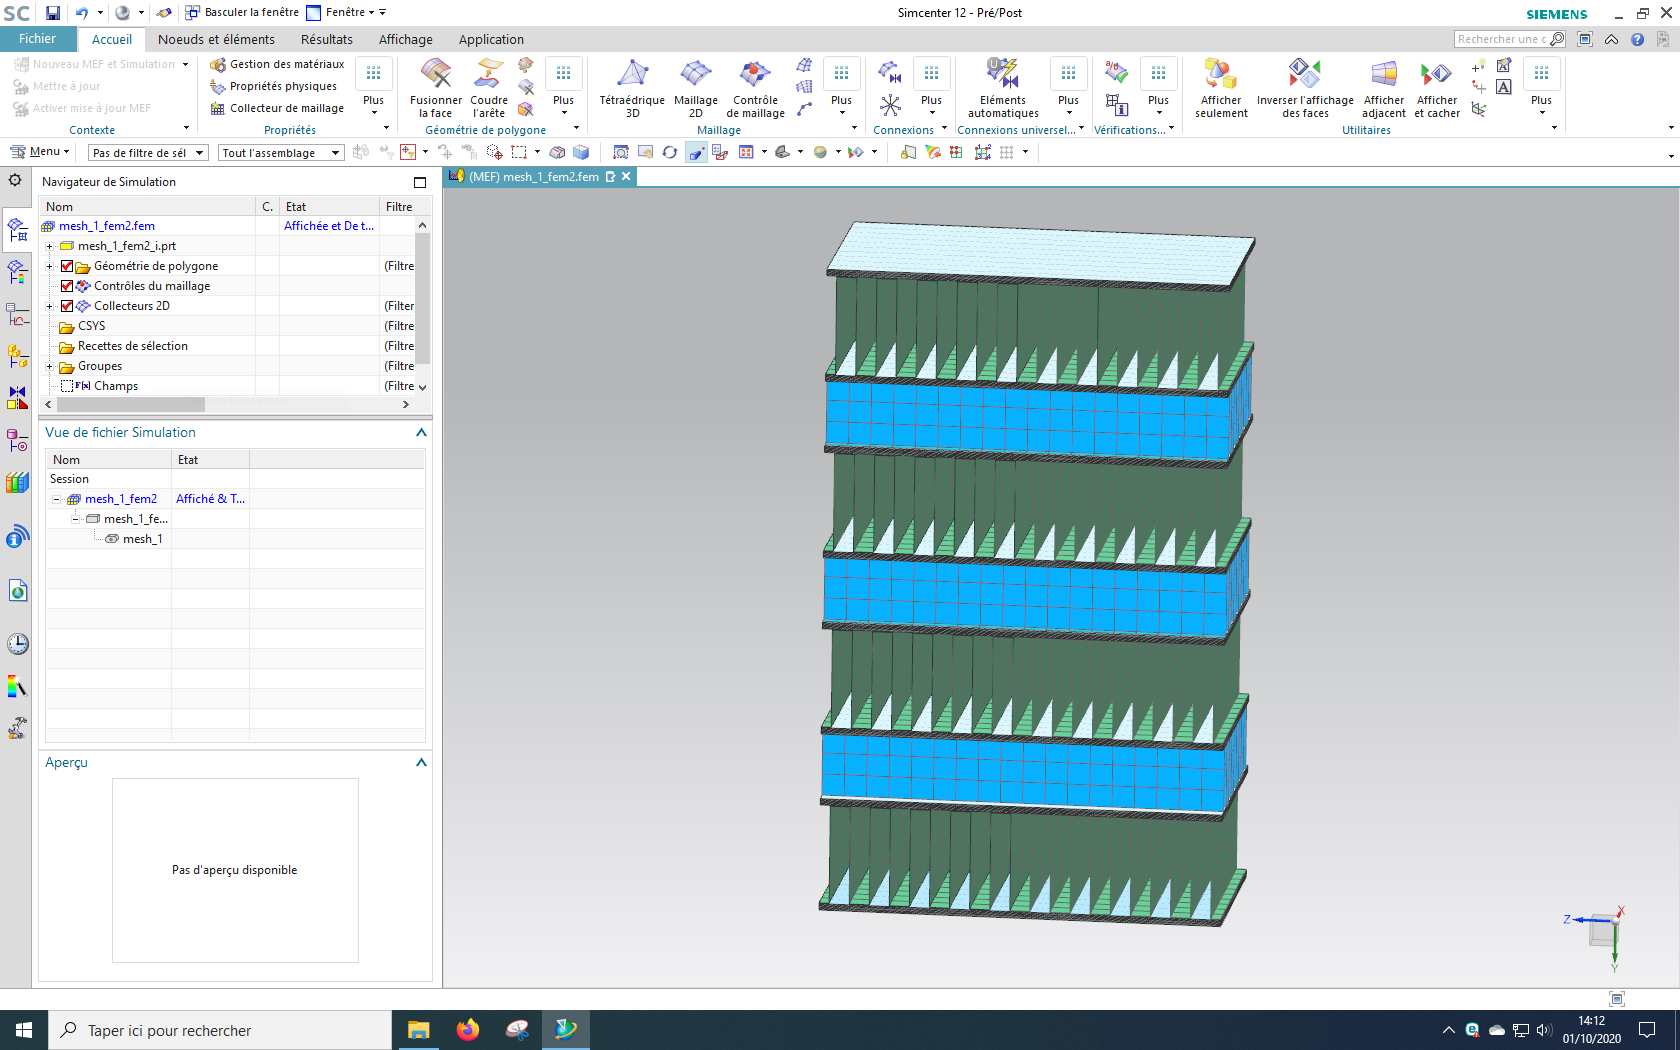
\includegraphics[scale=0.18]{SimcenterInterface.PNG}
      \caption{Interface du logiciel Simcenter 12 - vue active du modèle FEM}
         \label{SimcenterInterface}
\end{figure}

Néanmoins, l'utilisation de NX dans un journal python ne peut se faire presque uniquement que depuis l’interpréteur Python 3.64 intégré dans Simcenter et non un interpréteur configuré personnellement. Ceci veut dire que l'on a pas accès depuis Simcenter a toutes les autres bibliothèques externes, dont \textit{\textbf{NumPy}} ou \textit{\textbf{openTURNS}}, composants néanmoins nécessaires pour la génération de champs stochastiques et l'analyse de la pièce. \\

Pour contourner cette difficulté, le choix a été fait de scinder le programme en deux parties, une pour interagir directement avec Simcenter et le modèle de la pièce, faire l'analyse , exporter les résultats de l'analyse dans un fichier externe, et ensuite faire appel à un programme Python exécutable qui lui possède toutes les bibliothèques externes et génère les champs stochastiques et les déformations en fonction des données exportées. Ce second script enregistre à son tour toutes les données sur les déformation qui sont réimportés dans le premier script et les déformations appliqués. \\

Un schéma explicatif de la méthodologie et de l'architecture des codes se trouve en annexe. \\

\subsubsection{Commentaires et mise en contexte}

Bien que entièrement fonctionnel, la méthodologie mise en place se heurte encore à des limites externes. En effet, au cours du projet, des questionnement ont eu lieu quant à l'outil à utiliser pour les simulations thermo-mécaniques, et l'utilisation de Simcenter a été remise en question au profit du logiciel Altair.\\ 
Dans le cas ou le choix retomberait sur Altair, la méthodologie développée ne pourra plus être gardée, au vue des différences probablement importantes entre le langage de scriptage d'Altair et de Simcenter.\\ 
 
\subsection{Bilan intermédiaire}

Au vu des complications ayant étés entrainées par la pandémie de COVID-19, un ralentissement notable dans le secteur de l'aviation a eu des conséquences néfastes sur le projet, et celui a perdu de son importance immédiate chez Phimeca, comme chez les autres entreprises collaborant sur ce projet. 
Ce faisant, l'absence de données concernant l'échangeur de chaleur ont entravé sa modélisation, et des discussions avec les collaborateurs des autres entreprises ont soulevé des problèmes dans la modélisation initialement envisagée de l'échangeur. En effet, sans informations supplémentaires ni sur les moyens de fabrication employés, ni les matérieaux, ni sur les efforts exercés sur la pièce lors de son utilisation , nous ont empechés d'inclure certaines grandeurs physiques et efforts sur lesquels nous n'avions pas d'à-priori, notamment la masse intrinsèque au plaques, et la pose des plaques crenelées, qui, se faisant séquentiellement, vont graduellemrnt augmenter les efforts dans les niveaux de plaques inferieurs, et donc provoquer des déformation au fur et a mesure que le système est contruit. 

Nous avons donc décidé de mettre en pause cette partie du projet tant que des informations supplémentaires n'étaient pas obtenues, et de se concentrer sur l'intégration des codes et méthodes développés dans \textit{openTURNS}, comme de faire une étude plus en détail de l'example de la poutre en flexion, et de voir l'implication des différents paramètres de modélisation en jeu lors d'une telle analyse. 

\section{Derniers 5 mois de stage }
Comme mentionné précédemment, ces derniers mois de stage nous on permis de nous focaliser sur l'intégration des méthodes dans \textit{openTURNS}, tout comme d'analyser plus en détail cette méthode.

\subsection{Intégration dans openTURNS}
\subsubsection{Specifications pour l'intégration dans openTURNS}
Le but de la partie intégration, était de réecrire les codes de manière à ce qu'il y aie le plus possible de fonction internes à \textit{openTURNS} qui soient utilisées, de ne pas inclure d'autres librairies autres qu'\textit{openTURNS} et la librairie standard de \textbf{Python}, tout comme de rendre des codes documentés et lisibles, facilitant la transcription ensuite des codes dans le lanqage \textbf{C++}.

\subsubsection{Astuces employées pour l'intégration}
Puisque le choix a été fait de travailler dans un cas général de système pouvant prendre en entrée une combinaison arbitraire de lois aléatoires scalaires et de champs aléatoires a dimensions variables, et de retransformer le système de manière à ce qu'il ne prenne en entrée qu'un vecteur aléatoire normal centré réduit, l'utilisation des méthodes incluses dans \textit{openTURNS} était indispensable, notamment pour pouvoir traiter l'entierté des lois aléatoires présentes dans \textit{openTURNS}, tout comme tout type de champ stochastique, qu'il soit issu de lois de covariance, ou bien à partie d'une regression sur des données.

\begin{itemize}
  \item Pour permettre l'utilisation de tout type de champ, peu importe l'origine, l'idée était de travailler non pas sur le procéssus stochastique (qui est un objet à part dans \textit{openTURNS}) mais sur l'objet contenant la décomposition de Karhunen Loeve, appelé \textbf{KarhunenLoeveResults} dans l'API. 
  
  Cet objet permet de passer directement du vecteur centrée normal réduit au champ et inversemment. 
  \item Pour les lois aléatoires scalaires ceci est encore plus simple, puisque tout les lois scalaiers dans \textit{openTURNS} possèdent les méthodes \textbf{.IsoProbabilisticTransformation} et \textbf{.InverseIsoProbabilisticTransformation} qui permettent de passer d'une loi quelconque à une loi normale centrée réduite et inversment.
  
  \item Ces objets et méthodes combinées ont permis de créer le premier objet nécessaire à l'analyse de sensibilité sur champs stochastiques et a été appelé ici \textbf{AggregatedKarhunenLoeveResults}. Cet objet est crée en lui fournissant une liste ordonnée de \textbf{KarhunenLoeveResults} et de lois de distribution scalaires (il n'est pas possibile ici d'utiliser des lois composées, des vecteurs aléatoire ou encore des décompositions de procéssus stochastiques composés, puisque l'utilisation de tels objets ammenerait trop d'ambiguités). Ensuite cet objet offre la possibilité de transformer des vecteurs aléatoires centrés normaux réduits (ou ensemble de vecteurs appelés \textbf{samples}) en une liste de champs stochastiques et de variables scalaires, ou de faire cette transformation inverse. \emph{Cette modélisation soulève de nombreux problèmes pour le portage de ces codes dans le langage C++, en effet dans ce langage \textbf{il n'existe pas de conteneur semblable à une liste pouvant contenir des objets de différents types.} Cette contrainte impliquera qu'il faudra par-exemple séparer les différents objets et les indexer à part, et reconstruire la liste python dans une sur-couche adaptée.} 
  Cet objet serait entièrement nouveau dans l'environnement \textit{openTURNS}.
  
  \item Vu qu'une analyse de sensibilité s'appuie toujours sur une combinaison particulière de lois aléatoires et d'un système à anlyser, il fallait un moyen simple pour permettre de facilement changer des paramètres dans les lois aléatoires, sans pour autant compromettre l'interaction lois/modèle. En effet, changer des paramètres comme le seuil d'approximation (threshold) de la méthode de Karhunen-Loeve sur un champ stochastique a de très importants effets sur le nombre de modes à utiliser pour représenter le champ avec une telle précision (Dans le pire des cas, le nombre de modes serait égal au nombre d'élément contenus dans l'espace discretisé sur lequel on représente le champ). Ceci implique donc que le vecteur aléatoire qui pilote nos champs et variables scalaires est de taille variable, ce qui rend difficile, voire impossible de manuellement réecrire la fonction représentant notre système pour qu'elle prenne en entrée seulement le vecteur aléatoire. Ceci devient vraiment visible lorsqu'on cherche à faire une analyse de l'influence des paramètres des lois aléatoires sur l'analyse de Sobol', vu qu'à priori, à \textit{threshold} constant, tout combinaison différente de paramètrs des champs stochastiques va entrainer une longeur différente du vecteur aléatoire censé piloter notre système. 
  Ceci fait que dans la philosophie de cette méthode, on travaille surtout avec des fonctions prennant en entrée une liste de champs (appelés \textbf{Field} dans \textit{openTURNS}) et de variables scalaires, ou encore prennant en entrée une liste d'échantillons de champs et d'échantillons de points, si la fonction a été écrite pour traiter de nombreux cas en parallèle par exemple.
  Pour supprimer ce besoin de réecrire la fonction manuellement pour qu'elle prenne en entrée le vecteur aléatoire, on a crée un \textit{wrapper} qui permet de transformer la fonction du système réel en une nouvelle fonction ne prenant en entrée que ce vecteur aléatoire. Cet objet s'appelle \textbf{KarhunenLoeveGeneralizedFunctionWrapper} et prend en entrée le modèle "réel" et l'objet \textbf{AggregatedKarhunenLoeveResults} défini précedemment.
  
  \item Pour la partie analyse de sensibilité, nous utilisons la méthode classique basé sur une experience de monte-carlo, comme introduit dans la méthode issue du papier de \cite{Wei2017May}. La différence avec la méthode classique basée sur monte-carlo pour le calcul des indices de Sobol' est la manière de génerer la matrice des mélanges. Le schéma explicatif de ce mélange se trouve en figure \ref{expGenStoField}. L'implémantation de ce mélange se fait simplement, et peut facilement se traduire en C++. Pour la construction de l'objet permettant la génération d'échantillons, nous passons l'objet \textbf{AggregatedKarhunenLoeveResults}, la taille de l'échantillon et le booléen indiquant si l'on souhaite calculer les indices du second ordre ou non. Cette classe est appellée ici \textbf{KarhunenLoeveSobolIndicesExperiment}. Cette classe est conforme à la classe \textbf{SobolIndicesExperiment} dans \textit{openTUNRS}, pour un fonctionnement identique des codes. 
  
  \item Enfin, pour le calcul même des indices de Sobol', différentes méthodes existent. Pour n'en citer que celles qui sont implémentées dans \textit{openTURNS}, il y a la méthode de \textit{Martinez}, de \textit{Saltelli}, de \textit{Jansen} ou encore de \textit{Mauntz Kucherenko}. Comme ces méthodes utilisent uniquement la réponse du modèle aux valeurs contenues dans la matrice de mélange il n'y a à-priori pas besoin d'avoir des information concernant la matrice de mélange. Néanmoins, les classes pour le calcul des indices de Sobol' d'openturns, requierent en entrée la matrice de mélange, premièrement pour récuperer le nom des différentes variables, et vérifier si la dimension de la matrice de mélange est bien cohérente avec le nombre d'élement contenus dans la réponse du modèle, en se basant sur la formule $ N(2+d) $, \textbf{N} étant la taille de l'échantillon, et \textbf{d} la dimension du problème. Néanomins, avec la méthode impliquant la décomposition de Karhunen-Loeve, la dimension de la matrice de mélange 
  
  
  
  
  
  
   

\end{itemize}


\section{Conclusions}


\bibliography{Bibliographie_rapport_PHIMECA_Simady}

\appendix 
\appendixpage
\addappheadtotoc

\begin{figure}[H]
   \centering
   \vspace{-2cm}
   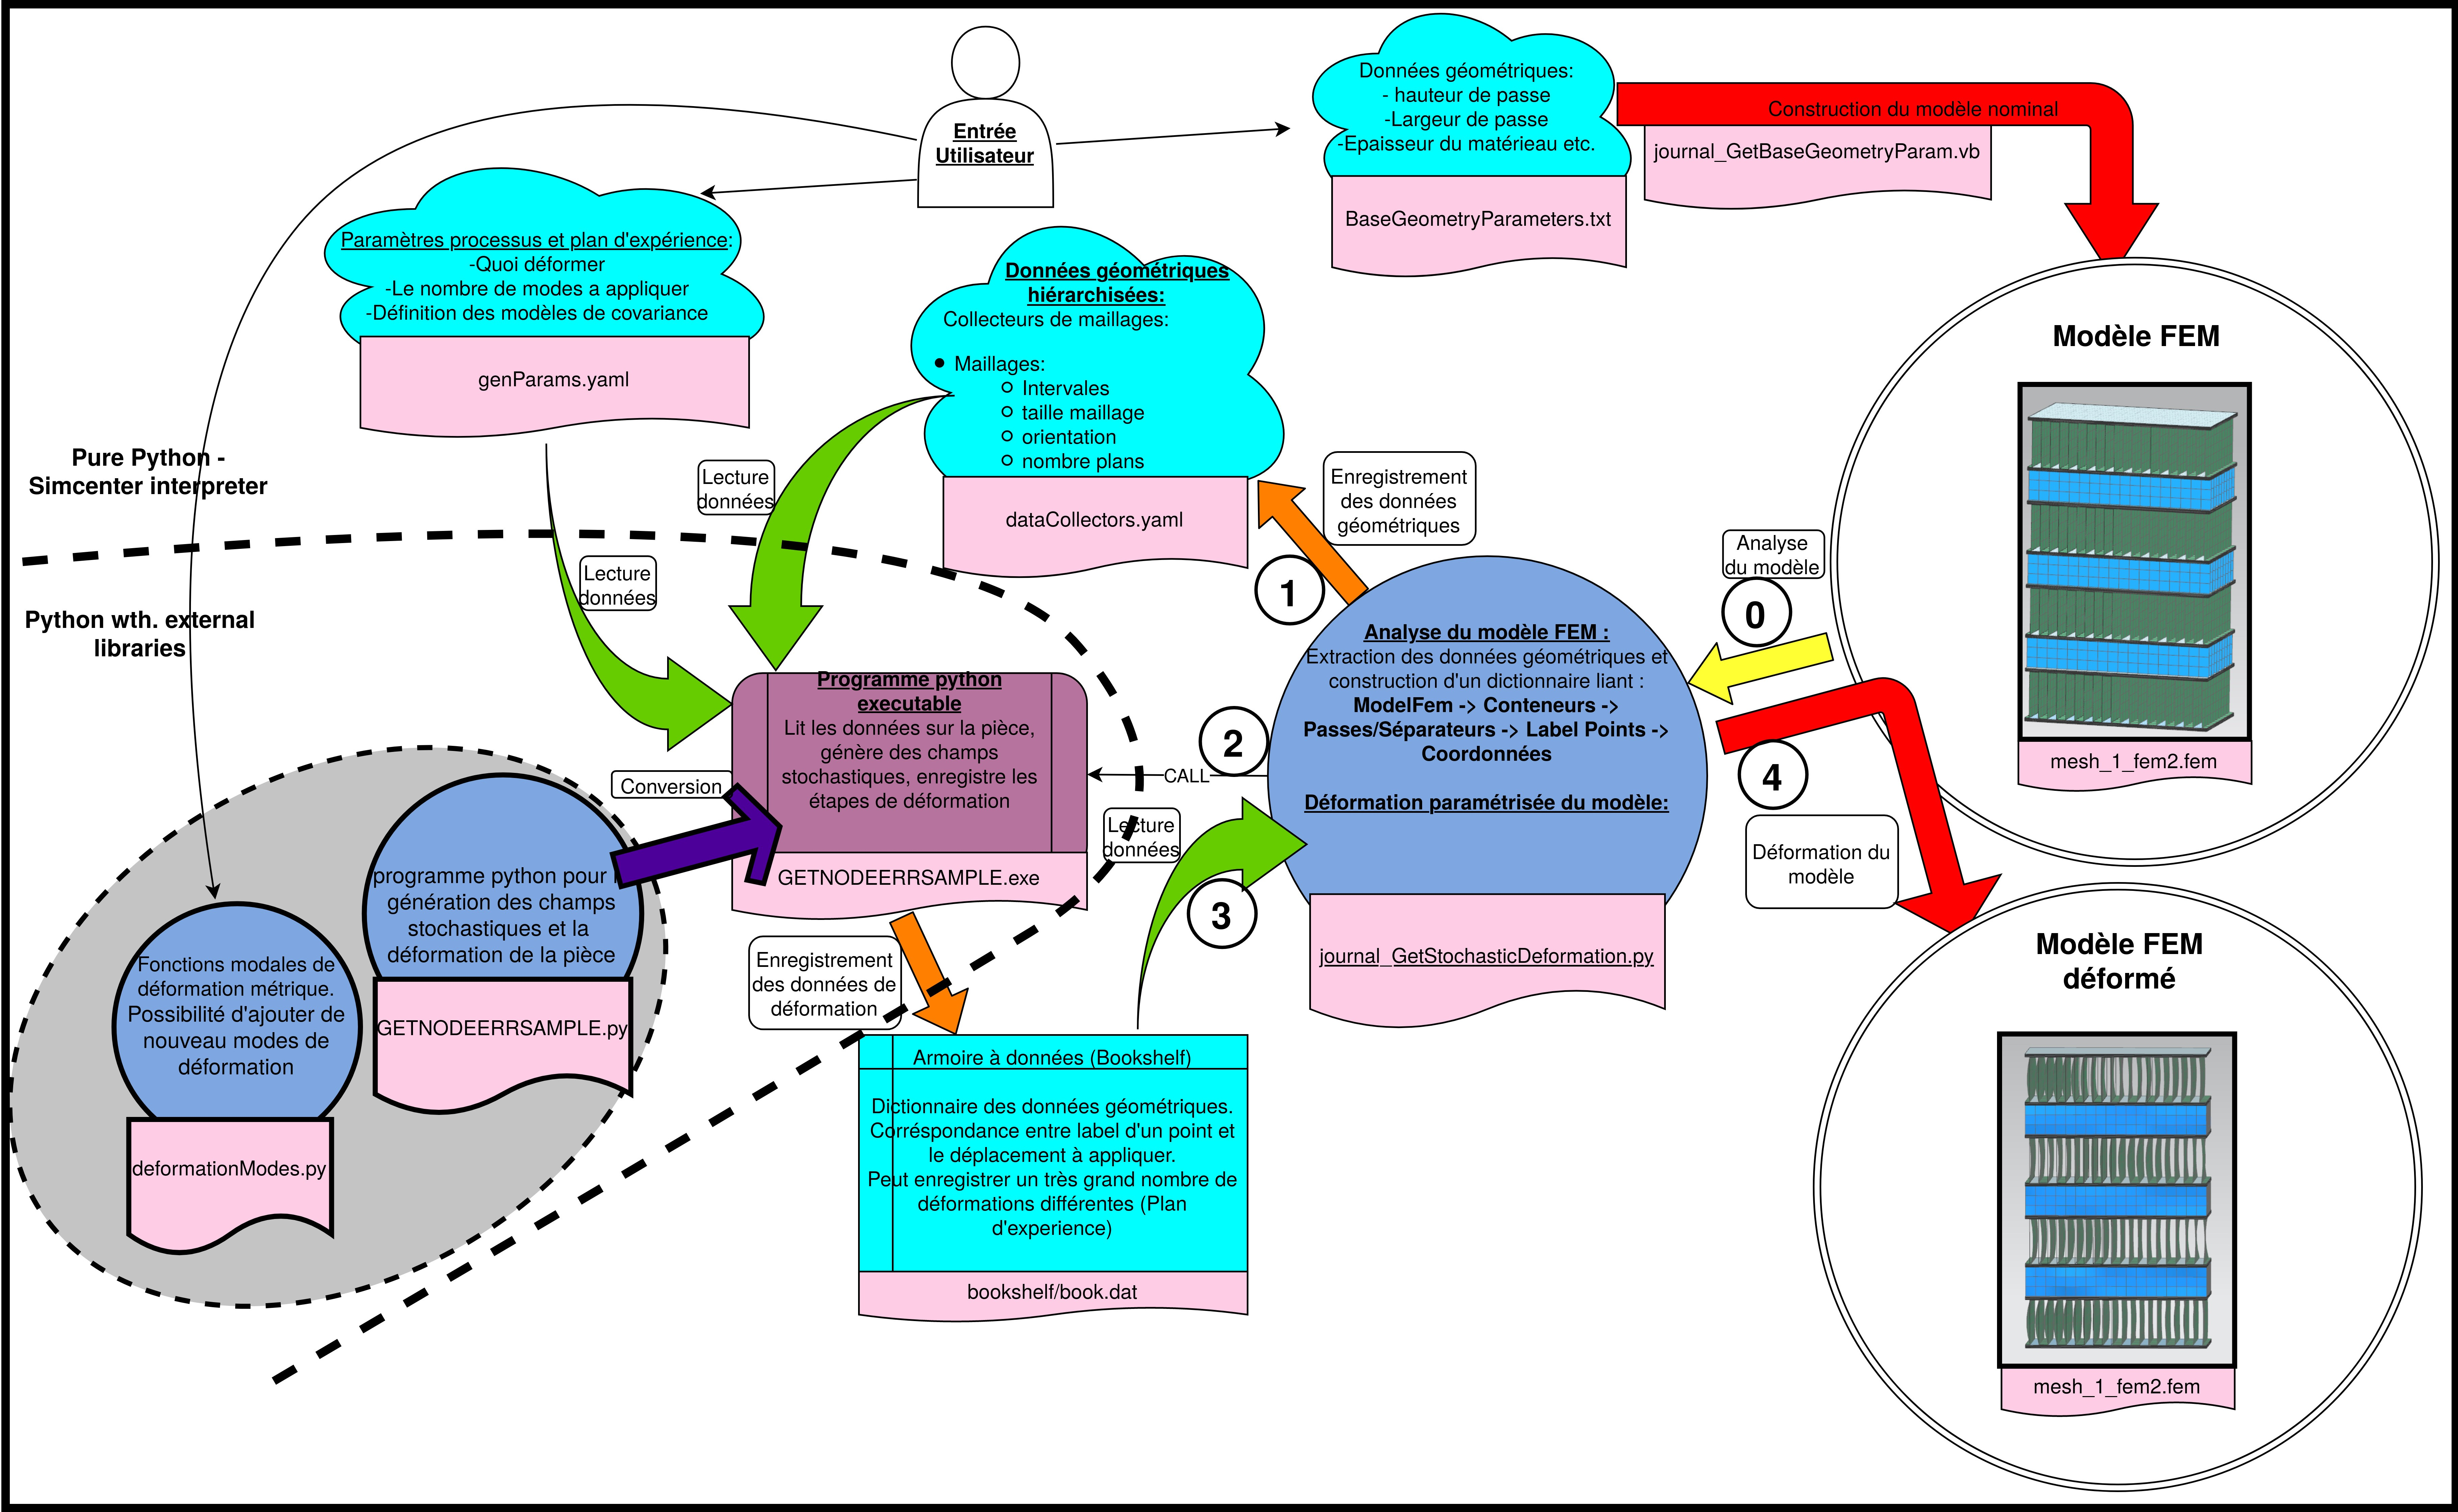
\includegraphics[angle=-90,origin=c,width=1.1\textwidth,height=1.1\textheight,keepaspectratio]{SchemaDeformationNastran.jpg}
      \caption{Architecture des programmes servant à introduire des déformations pilotées par champ stochastique dans l'échangeur de chaleur}
         \label{SchemaDeformationNastran}
\end{figure}

\end{document}

